\documentclass{thesisclass}
% Based on thesisclass.cls of Timo Rohrberg, 2009
% ----------------------------------------------------------------
% Thesis - Main document
% ----------------------------------------------------------------

\usepackage{listings}
\usepackage{acronym}
\usepackage{amsmath}

% Breaks in equation
\usepackage{breqn}

%% -------------------------------
%% |  Information for PDF file   |
%% -------------------------------
\hypersetup{
 pdfauthor={Not set},
 pdftitle={Not set},
 pdfsubject={Not set},
 pdfkeywords={Not set}
}


%% -------------------------------
%% |   New Title Page Info       |
%% -------------------------------

\newcommand{\docType}{Bachelor Thesis} % select your thesis type
\newcommand{\mainTitle}{Design, Implementation and \\ eval\nolinebreak uation of different strategies for playing Pokémon battles}

\newcommand{\authorName}{Julian Schubert}

\newcommand{\reviewerOneName}{Prof. Dr. Frank Puppe}
\newcommand{\reviewerOneTask}{First Reviewer}

\newcommand{\advisorOneName}{Jonathan Krebs}
\newcommand{\advisorOneTask}{First Advisor}

% if only one advisor remove next two lines
%\newcommand{\advisorTwoName}{Name Advisor 2}
%\newcommand{\advisorTwoTask}{Second Advisor}

% if no external advisor remove next two lines
%\newcommand{\advisorExtName}{Name External Advisor}
%\newcommand{\advisorExtTask}{External Advisor}

\newcommand{\submissionTime}{XX. Month 20YY}

%% -------------------------------
%% | Information for Declaration |
%% -------------------------------
\newcommand{\place}{Place}

%% ---------------------------------
%% | ToDo Marker - only for draft! |
%% ---------------------------------
% Remove this section for final version!
\setlength{\marginparwidth}{20mm}

\newcommand{\margtodo}
{\marginpar{\textbf{\textcolor{red}{ToDo}}}{}}

\newcommand{\todo}[1]
{{\textbf{\textcolor{red}{(\margtodo{}#1)}}}{}}


%% --------------------------------
%% | Old Marker - only for draft! |
%% --------------------------------
% Remove this section for final version!
\newenvironment{deprecated}
{\begin{color}{gray}}
{\end{color}}


%% --------------------------------
%% | Settings for word separation |
%% --------------------------------
% Help for separation:
% In german package the following hints are additionally available:
% "- = Additional separation
% "| = Suppress ligation and possible separation (e.g. Schaf"|fell)
% "~ = Hyphenation without separation (e.g. bergauf und "~ab)
% "= = Hyphenation with separation before and after
% "" = Separation without a hyphenation (e.g. und/""oder)

% Describe separation hints here:
\hyphenation{
% Pro-to-koll-in-stan-zen
% Ma-na-ge-ment  Netz-werk-ele-men-ten
% Netz-werk Netz-werk-re-ser-vie-rung
% Netz-werk-adap-ter Fein-ju-stier-ung
% Da-ten-strom-spe-zi-fi-ka-tion Pa-ket-rumpf
% Kon-troll-in-stanz
}


%%%%%%%%%%%%%%%%%%%%%%%%%%%%%%%%%
%% Here, main documents begins %%
%%%%%%%%%%%%%%%%%%%%%%%%%%%%%%%%%
\begin{document}

% Remove the following line for German text
\selectlanguage{english}

\frontmatter
\pagenumbering{roman}
\begin{titlepage}

\setmarginsrb{0mm}{0mm}{0mm}{0mm}{0mm}{0mm}{0mm}{0mm}


\begin{tikzpicture}[remember picture,overlay]
    \node [inner sep=0pt] (background_img) at (15, -17) {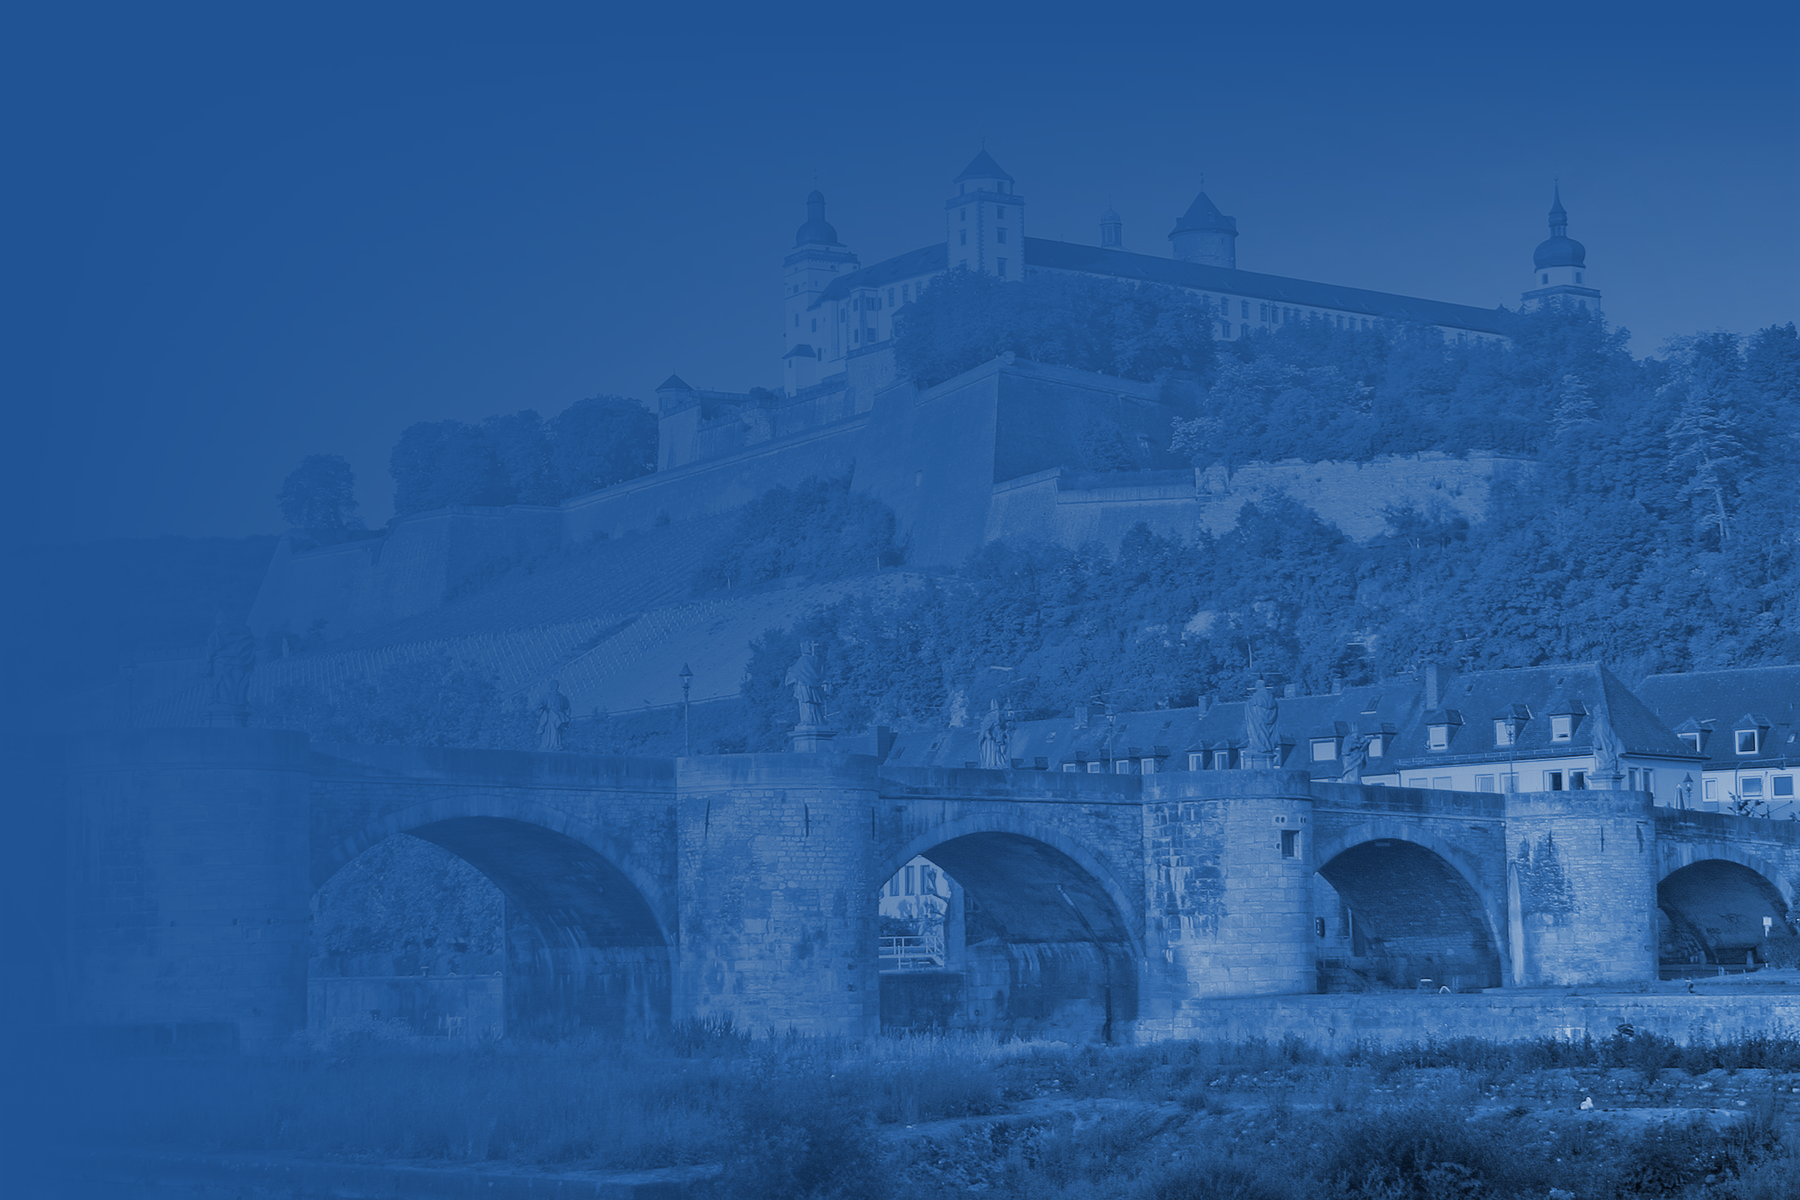
\includegraphics[width=38cm]{logos/Marienberg_wuerzburg_verlauf.png}};
    \node [fill=white, minimum width=133mm, minimum height=600mm] (box) at (current page.north west){};
    \node [inner sep=0pt] (uniwuelogo) at (12.98,-5) {
\includegraphics[width=\paperwidth]{logos/unilogo4c_gross.png}};
\end{tikzpicture}

\pagecolor{background}

\begin{textblock*}{170mm}(80mm,45mm)
    \noindent
    \renewcommand{\baselinestretch}{1.5}
    \huge\textsf{\textcolor{titlecolor}{\docType}}
\end{textblock*}

% Title
\begin{textblock*}{130mm}(80mm,95mm)
    \noindent
    \Huge\textsf{\textbf{\textcolor{titlecolor}{\mainTitle}}}
\end{textblock*}


% First author
\begin{textblock*}{120mm}(80mm,175mm)
    \noindent
    \Large\textsf{\textcolor{titlecolor}{
    \textbf{\authorName} \\
    \authorDepartment\\
    \authorChair
    }}
\end{textblock*}

\ifdefined\advisorTwoName
	% case 1: one reviewer and two advisor
	% First reviewer
\begin{textblock*}{120mm}(80mm,220mm)
	\noindent
	\Large\textsf{\textcolor{titlecolor}{
			\textbf{\reviewerOneName} \\
			\reviewerOneTask
	}}
\end{textblock*}


% First advisor
\begin{textblock*}{120mm}(80mm,235mm)
	\noindent
	\Large\textsf{\textcolor{titlecolor}{
			\textbf{\advisorOneName} \\
			\advisorOneTask
	}}
\end{textblock*}

% second advisor
\begin{textblock*}{120mm}(80mm,250mm)
	\noindent
	\Large\textsf{\textcolor{titlecolor}{
			\textbf{\advisorTwoName} \\
			\advisorTwoTask
	}}
\end{textblock*}

\ifdefined\advisorExtName
	% external advisor
	\begin{textblock*}{120mm}(80mm,265mm)
		\noindent
		\Large\textsf{\textcolor{titlecolor}{
			\textbf{\advisorExtName} \\
			\advisorExtTask
		}}
	\end{textblock*}
\fi	
	
\else
	% case 2: one reviewer and one advisor
		% First reviewer
	\begin{textblock*}{120mm}(80mm,220mm)
		\noindent
		\Large\textsf{\textcolor{titlecolor}{
				\textbf{\reviewerOneName} \\
				\reviewerOneTask
		}}
	\end{textblock*}
	
	% First advisor
	\begin{textblock*}{120mm}(80mm,235mm)
		\noindent
		\Large\textsf{\textcolor{titlecolor}{
				\textbf{\advisorOneName} \\
				\advisorOneTask
		}}
	\end{textblock*}
\ifdefined\advisorExtName
	% external advisor
	\begin{textblock*}{120mm}(80mm,250mm)
		\noindent
		\Large\textsf{\textcolor{titlecolor}{
			\textbf{\advisorExtName} \\
			\advisorExtTask
		}}
	\end{textblock*}
\fi
\fi
% Date
\begin{textblock*}{60mm}(80mm,305mm)
    \noindent
    \Large\textsf{\textcolor{titlecolor}{\textbf{Submission\\}\submissionTime}}
\end{textblock*}

% Webadress
\begin{textblock*}{110mm}(115mm,311mm)
    \noindent
    \hfill\Large\textsf{\textcolor{titlecolor}{\textbf{\webadress}}}
\end{textblock*}

\end{titlepage}

\nopagecolor
% reset margins to standrad for text
\setmarginsrb{3cm}{1cm}{3cm}{1cm}{6mm}{7mm}{5mm}{15mm}
\blankpage
\chapter*{Abstract}
Pokémon is the highest-grossing video game franchise and revolves around collecting Pokémon with the 
ultimate goal of becoming \grqq the very best, like no one ever was\grqq. This thesis provides a detailed
introduction to competitive Pokémon battles and summarizes previous research on the topic. Current
search-based agents lack proper long term planning as the large quantity of possible states limits
the amount of turns that can be looked ahead. A combination of existing \textit{MiniMax}-
and rule based-agents that allows for planning and execution of a match plan is introduced.
After playing over 1,400 battles on the \textit{Pokémon Showdown} ranked ladder against human players,
the bot achieved a mean Elo of $1,227$ and a maximum of $1,432$. While the agent only won 273 out of 
1,000 games against the best open source implementation, analysis of battles lead to the conclusion that defeats
are often caused by lack of features that due to time restrictions were not fully implemented. 
Additionally, the initial state of over 70,000 games was rated and then played out by two baseline 
agents. Results showed that both a random agent and an agent that prioritizes the most damaging
move have a lower win rate on unfavorable board ratings while winning more games on a positive rating. 

%!TEX root = thesis.tex

\chapter*{Zusammenfassung}
\selectlanguage{ngerman}


% this is the last line of the file
\selectlanguage{english}



%% -------------------
%% |   Directories   |

%% -------------------
% set the table of contents depth (= section levels which should be included in TOC)
\setcounter{tocdepth}{2}
\tableofcontents
\blankpage


%% -----------------
%% |   Main part   |
%% -----------------
\mainmatter
\pagenumbering{arabic}
%!TEX root = thesis.tex

\chapter{Introduction}
\label{ch:introduction}

\begin{wrapfigure}{r}{0.5\textwidth}
    \begin{center}
      
\includegraphics[width=0.48\textwidth]{images/pikachu.png}
    \end{center}
    \caption{Pikachu, one of the most popular Pokémon~\autocite{Fandom:AshsPikachu}}
    \label{fig:pikachu-image}
\end{wrapfigure}
Pokémon (an abbreviation for \textbf{Pocket Monsters}) is a media franchise managed my \textit{The Pokémon Company}, a company
founded by \textit{Nintendo}, \textit{Game Freak} and \textit{Creatures}~\autocite{Wikipedia:Pokemon}. Figure \ref{fig:pikachu-image} shows an image of
\textit{Pikachu}, one of the most popular Pokémon. Among multiple movies and series, a large variety of Pokémon games was released, starting with
\textit{Pokémon Red} and \textit{Pokémon Blue} which were released on the 28. September 1998, also known as \ac{GEN1}-games. In order to promote
trading between players, \textit{Nintendo} publishes two very similar games at the same time. 
Both releases differ in a few minor story differences and in the available Pokémon. Therefore, in order to collect all available Pokémon,
players either have to buy two copies of the game or trade with a player that owns the counterpart. As of writing, there are eight major
releases, also called \textit{mainline games} with the latest being \textit{Pokémon Sword} and \textit{Pokémon Shield}. While the graphics
evolved a lot over the years (see figures \ref{fig:red0}, \ref{fig:red1}, \ref{fig:sword0} and \ref{fig:sword1}), the key concept of the 
game remained mostly unchanged.
\begin{figure}[ht]
  \centering
  \begin{minipage}{.5\textwidth}
    \centering
    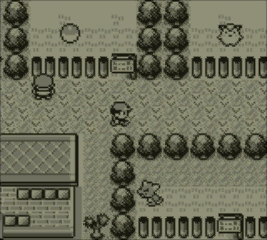
\includegraphics[width=.95\linewidth]{images/Red-0.jpg}
    \captionof{figure}{Exploring the map in \\Pokémon Red}
    \label{fig:red0}
  \end{minipage}%
  \begin{minipage}{.5\textwidth}
    \centering
    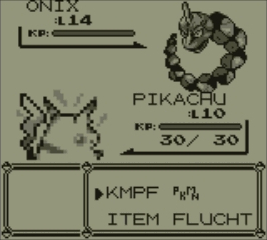
\includegraphics[width=.95\linewidth]{images/Red-1.jpg}
    \captionof{figure}{Fighting another trainer in \\Pokémon Red}
    \label{fig:red1}
  \end{minipage}
  \caption*{Image source: \href{https://www.nintendo.de/Spiele/Game-Boy/Pokemon-Rote-Edition-266109.html}{nintendo.de}}
\end{figure}
The player starts his journey in his hometown to become \textit{Pokémon Champion} which is the highest known 
level of rank for a Pokémon trainer \todo{https://bulbapedia.bulbagarden.net/wiki/Pokémon_Champion}. In order
to achieve this goal, the player has to create a team of up to six individual Pokémon which he then trains 
to unleash their full potential. 
\begin{figure}
  \centering
  \begin{minipage}{.5\textwidth}
    \centering
    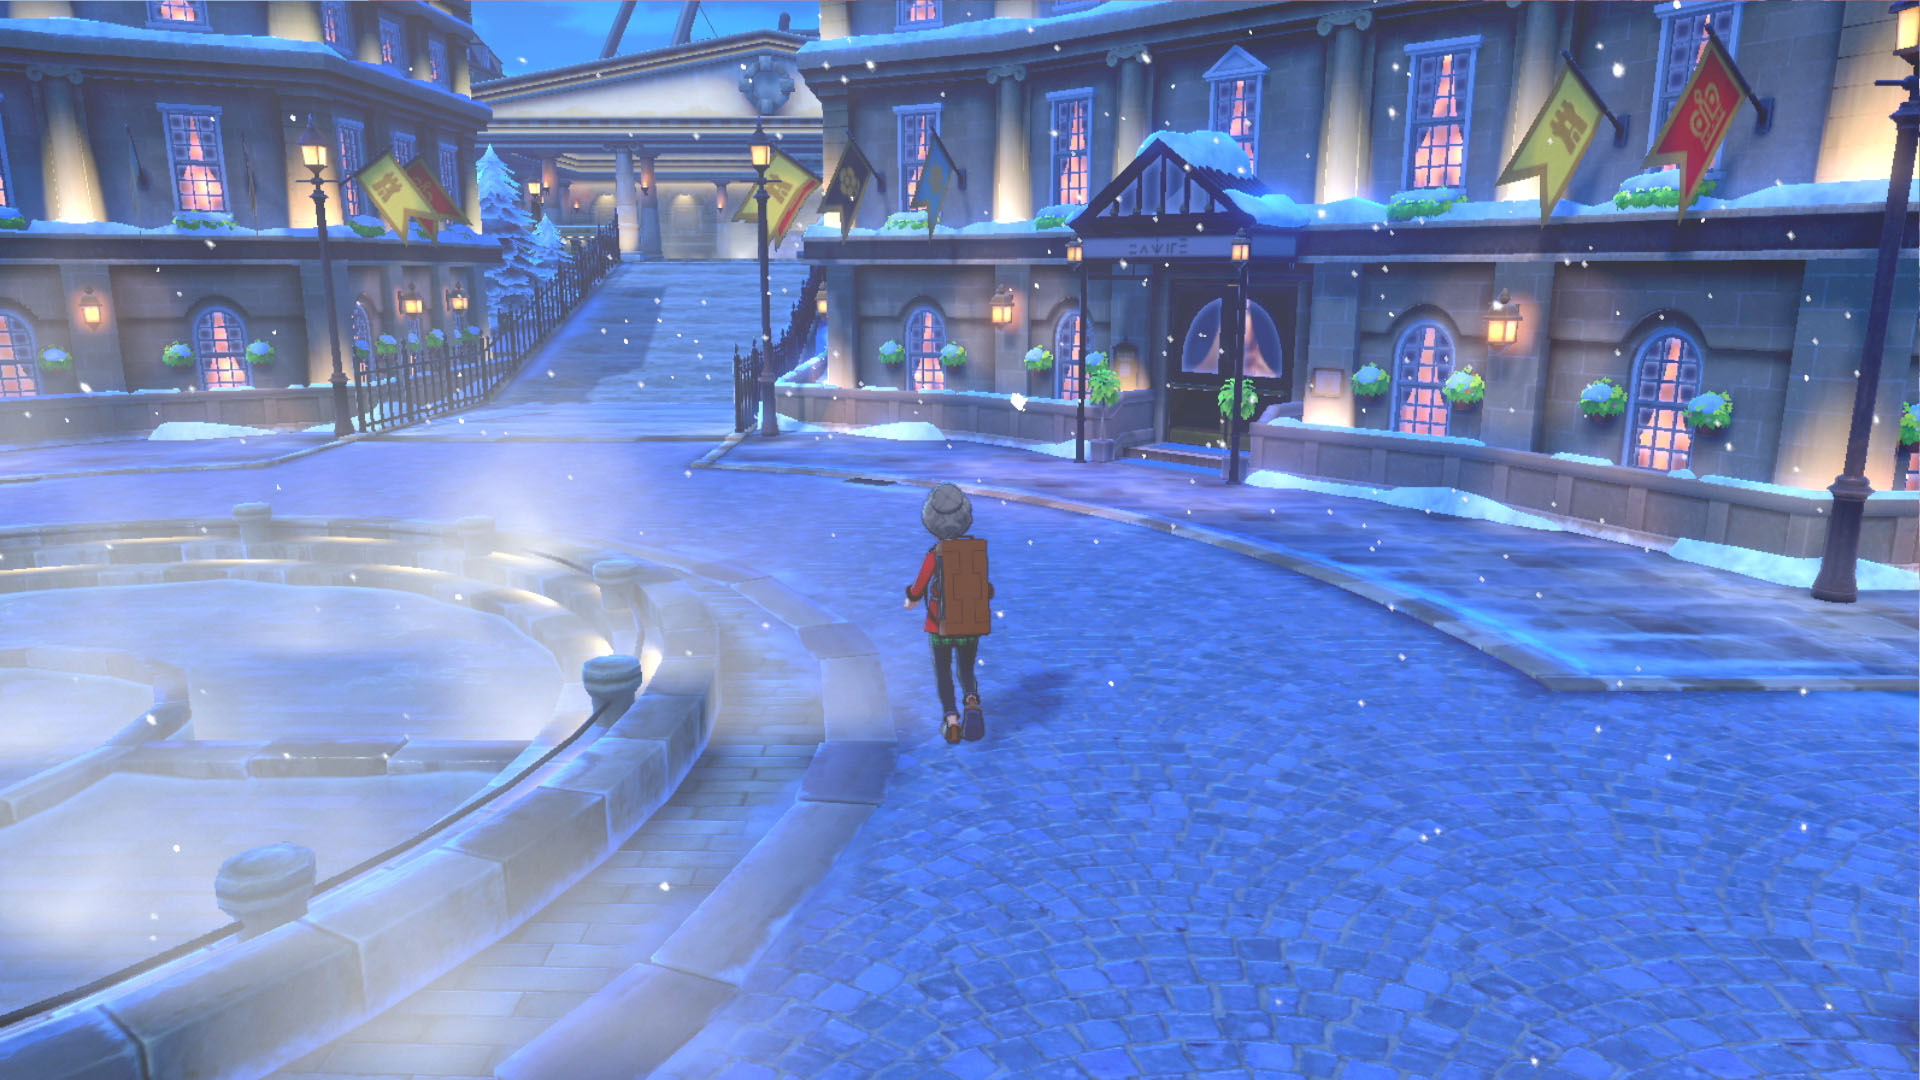
\includegraphics[width=.95\linewidth]{images/Sword-0.jpg}
    \captionof{figure}{Exploring the map in \\Pokémon Sword. \\ 
      Image source: \href{https://swordshield.pokemon.com/de-de/gameplay/pokemon-battle-stadium/}{pokemon.com}}
    \label{fig:sword0}
  \end{minipage}%
  \begin{minipage}{.5\textwidth}
    \centering
    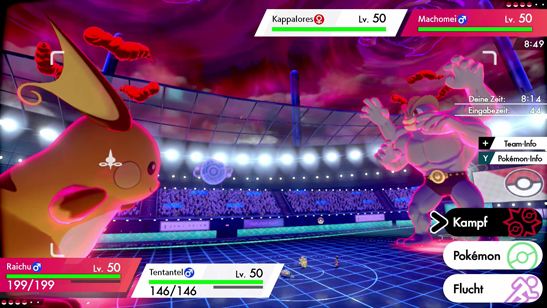
\includegraphics[width=.95\linewidth]{images/Sword-1.jpg}
    \captionof{figure}{Fighting another trainer in \\Pokémon Sword \\
      Image source: \href{https://www.nintendo.de/Spiele/Nintendo-Switch/Pokemon-Schwert-1522111.html}{nintendo.de}}
    \label{fig:sword1}
  \end{minipage}
\end{figure}
This Thesis focuses exclusively on the battling aspect of the game as there are detailed lists of locations and
secrets there is to explore within the games. Pokémon battles are turn based where both players, unlike in 
for example chess, make their decisions at the same time. While the core battle mechanics are very simple, 
the game provides a lot of depth which lead to the formation of a strong competitive battling scene.
As catching training Pokémon to a level where they are competitive viable is a time-intensive task, battle
simulators like  the open source project \textit{Pokémon Showdown} \todo{Cite} have arisen. On these fan made
platforms, players have access to all available Pokémon and can compete against each other in a large variety
of formats.
\begin{figure}
  \centering
  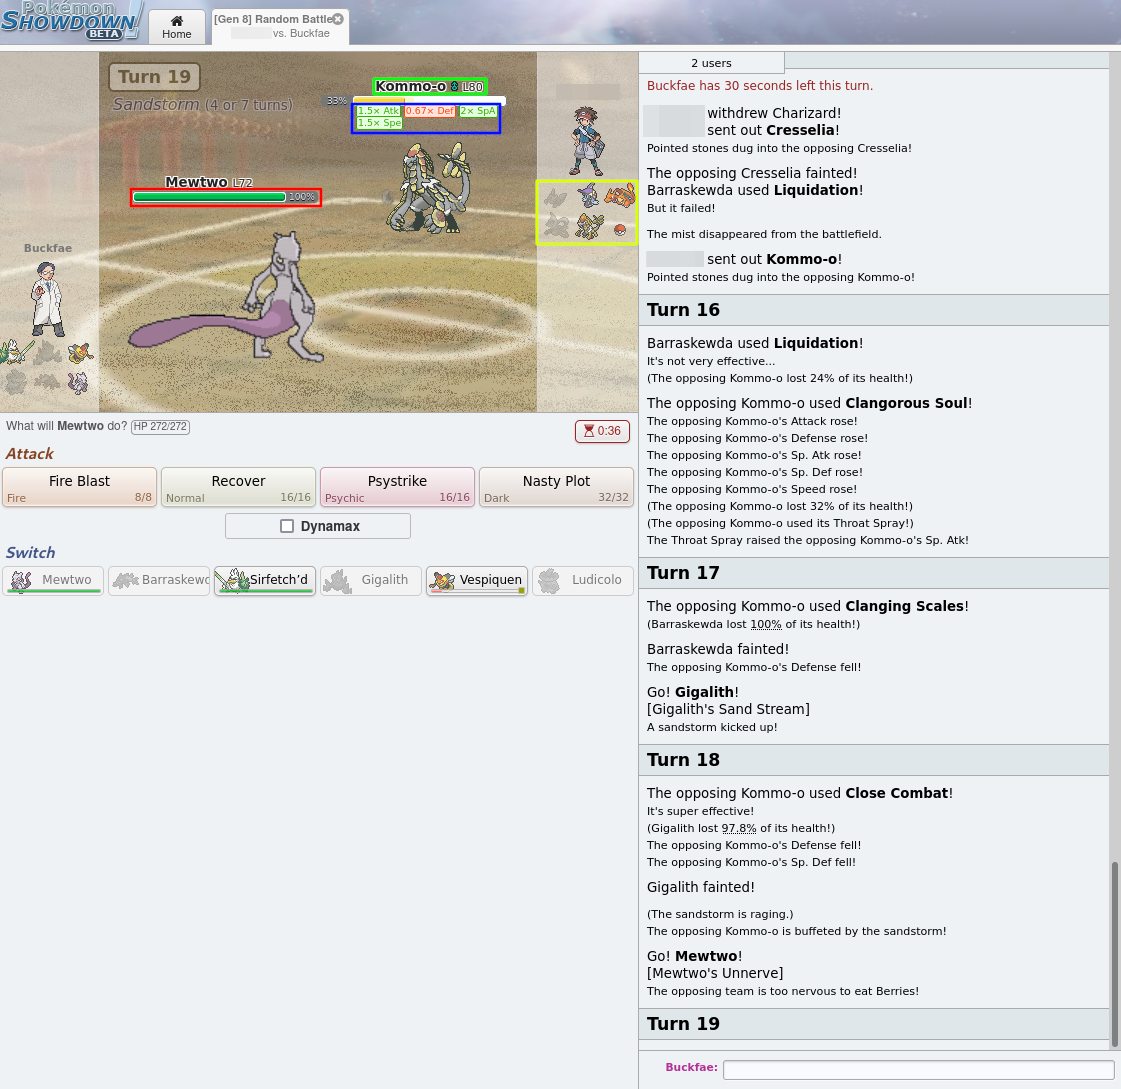
\includegraphics[width=1\textwidth]{images/Showdown.png}
  \caption{Battle between two players on \textit{Pokémon Showdown}}
  \label{fig:showdown-battle}
\end{figure}
Figure \ref{fig:showdown-battle} \todo{Move figure to appendix} shows a battle between two players on 
\textit{Pokémon Showdown}. The screenshot was taken from a \textit{Gen 8 random battle} between 
\textit{Buckfae} and another player\footnote{The other name was blurred}. The screenshot was taken
at the start of turn 19. Currently, the \textit{Mewtwo} of \textit{Buckfae} is at full health (indicated
red) while the opposing \textit{Kommo-o} has 33\% of \ac{HP} remaining. Below the avatars of both players,
the remaining team is displayed, marked yellow for player two. While player one has three Pokémon remaining,
his opponent has four members alive. The Pokéball (bottom right) indicates an to the player unknown Pokémon.
Lastly, the blue box highlights the status modifications of the enemy Pokémon. The effects of status conditions
will be covered in detail in section \todo{Link to status}. Below the game window, the possible choices of the
player are displayed. \textit{Mewtwo} has access to the moves \textit{Fire Blast}, \textit{Recover}, \textit{Psystrike}
and \textit{Nastyplot}. In addition to \textit{Dynamaxing} which will be coverd in \todo{Link to dynamax} the player
also has the option to switch to any of his remaining Pokémon \textit{Sirfetch'd} or \textit{Vespiquen}. Lastly,
on the right-hand side a log of the previous turns can be found. In addition to the moves a Pokémon can use,
a Pokémon has one ability and can hold an item that yields advantages in battle. \\
As game states in Pokémon are high-dimensional with the majority of features being both categorical and 
partially observable, Pokémon battles present a worthy challenge for AI to tackle \todo{I stole parts
of this sentence from somewhere, no idea where. Can I keep it?}.

\chapter{Background}

\section{Basic rules}
\todo{Explain Dynamaxing!}
\section{Battling}
\label{sec:battling}
One of the key aspects of the Pokémon game is to battle other Pokémon. In the mainline games, you can 
have up to six Pokémon in your team, also known as party. There is the option to swap a Pokémon with
another Pokémon, but you can not have more than six Pokémon at any point in your team. When playing the 
original games, you explore the world to find more Pokémon and use your team to defeat wild Pokémon
and other Pokémon trainers. This thesis focuses on random battles taking place on Pokémon Showdown.
In a random battle, both competitors get a team of six random Pokémon. At the start of the battle,
you know each of your six Pokémon but only the currently active enemy Pokémon. \\
In every turn, both players can choose to either use a move of their currently active Pokémon or switch
their active Pokémon to another Pokémon. Moves can either deal direct damage to the enemy Pokémon or 
yield other advantages like increasing the damage dealt by the next move. Moves will be covered in more
detail in section \ref{sec:moves}. Each Pokémon has an amount of \ac{HP}. The \ac{HP} of a Pokémon
can be dropped by attacking it with a move. If the \ac{HP} of a Pokémon drops to zero, it faints and 
can not be used in this battle anymore. A player wins, once all enemies fainted. \\
Note that in the mainline games there is the possibility to heal or even revive a fainted 
Pokémon during battle using \textit{Healing Items} like \textit{Revive} or \textit{Hyper Potion}.
In competitive Play, only \textit{Held items} like \textit{Leftovers} are allowed. Items will be explained
in depth in section \ref{sec:items}.

\subsection{Types}
\label{sec:types}
Pokémon implements a \ac{RPS}-like system. Each Pokémon has either one or two of 
18 types. Like \emph{rock} beats \emph{scissors} but looses to \emph{paper}, \textit{Fire}-type Pokémon have an
\textit{advantage} against \textit{Grass}-type Pokémon but are on a \textit{disadvantage} against \textit{Water}-types.
This is also called a type being \textit{strong} / \textit{weak} against another type.
\begin{figure}
	\centering
	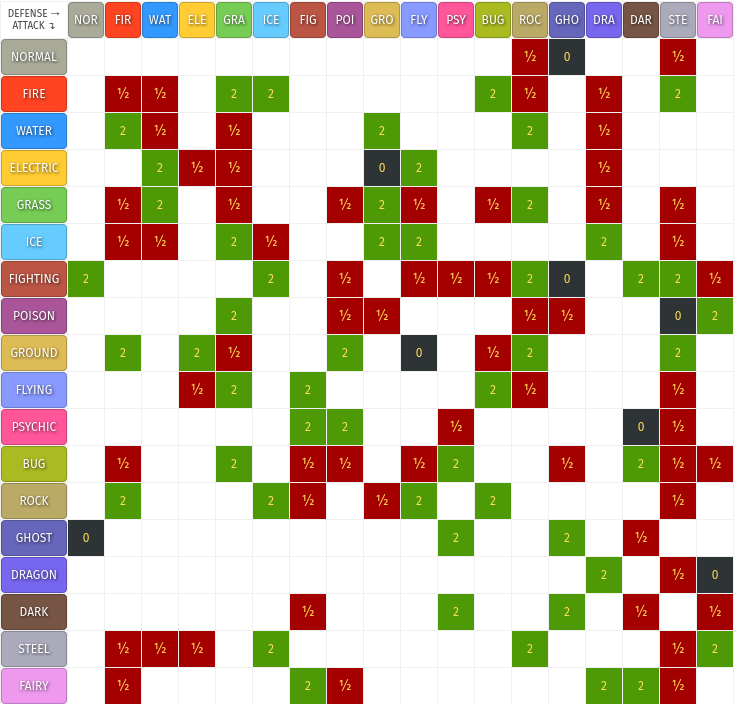
\includegraphics[width=0.7\textwidth]{images/type_chart.png}
	\caption{Advantages of different types ~\autocite{Pokemondb:Type}}
	\label{fig:type_chart}
\end{figure}
Figure \ref{fig:type_chart} shows how different Pokémon types interact with each other.
Unlike in \ac{RPS}, type modifiers will be multiplied if a Pokémon has two types. For instance, a \textit{Fire}-type
attack will deal 4 times the damage against \textit{Parasect} as \textit{Parasect} has the types \textit{Grass} and
\textit{Bug} ~\autocite{Veekun:Parasect}.

\subsection{Moves}
\label{sec:moves}
Moves can be split up into three categories: \textit{Physical}-, \textit{Special}- and \textit{Status}-Moves.
While \textit{Physical}- and \textit{Special}-Moves usually deal damage to the opponent Pokémon, 
\textit{Status}-Moves can for example change the weather, which plays a role in damage calculation explained
in section \ref{sec:damage-calculation}, inflict status effects, raise or lower the stats of a Pokémon. In 
addition, a move also has exactly one of the 18 possible types. Often, \textit{Status}-moves are also referred
to as \textit{buffing} moves if they grant a benefit to the user or as \textit{debuffing} if they have a
negative effect on the opponent.

\subsection{Pokémon}
\label{sec:pokemon}
\todo{High level explanation of Pokémon?}
A key-concept of Pokémon battles are the \textit{stats} of a Pokémon. 
\begin{figure}[h]
	\centering
	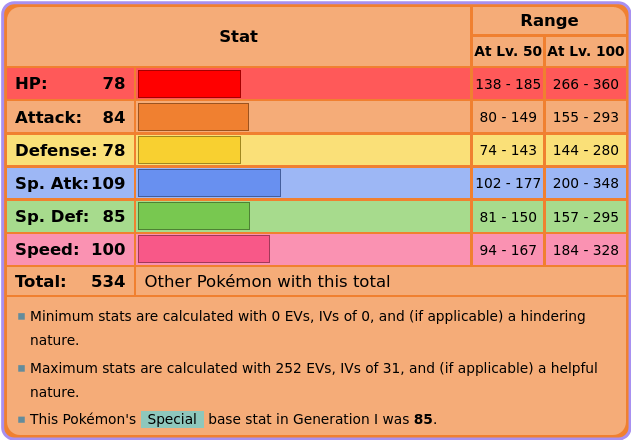
\includegraphics[width=0.7\textwidth]{images/charizard-stats.png}
	\caption{Possible stats of \textit{Charizard} ~\autocite{Bulbapedia:Charizard}}
	\label{fig:charizard-stats}
\end{figure}
Figure \ref{fig:charizard-stats} displays information about possible stat-combinations of 
\textit{Charizard}. 
\paragraph{Explanation of stats}
\textbf{HP:} The \ac{HP} determines how much damage a Pokémon can receive before fainting. \\
\textbf{Attack:} The \ac{ATK} determines how much damage a Pokémon will deal when using 
a \textit{Physical}-Move. \\
\textbf{Defense:} The \ac{DEF} determines how well a Pokémon can resist against \textit{physical} attacks. \\
\textbf{Sp. Atk:} The \ac{SPA} determines how much damage a Pokémon will deal when using
a \textit{Special}-Move. \\
\textbf{Sp. Def:} The \ac{SPD} determines how well a Pokémon can resist against special attacks. \\
\textbf{Speed:} The \ac{SPE} determines how fast a Pokémon can act. Usually, the Pokémon with a higher
\ac{SPE} will move before the slower one. The exact order of actions in battles is covered in section
\ref{sec:order-of-events}.
\todo{Cover evasion / accuracy, context to showdown}

\paragraph{Determination of stats}
\label{sec:stat-calculation}
The total stat of a Pokémon is calculated as described in equation \ref{eq:stats-hp} and equation 
\ref{eq:stats-other} ~\autocite{Bulbapedia:Stat}.
\begin{equation}
	\label{eq:stats-hp}
	HP = \Bigl\lfloor \frac{(2 \times Base + IV + \lfloor \frac{EV}{4} \rfloor) \times Level}{100}\Bigr\rfloor
	+ Level + 10 \\
\end{equation}
\begin{equation}
	\label{eq:stats-other}
	OtherStat = \Bigl\lfloor \Big( \frac{2 \times Base + IV + \lfloor \frac{EV}{4} \rfloor) \times Level}
	{100} + 5\Big) \times Nature \Bigr\rfloor
\end{equation}
\textbf{Base:} Refers to the base stat of a Pokémon. Two Pokémon of the same species will always have the 
same base-stats. As seen in figure \ref{fig:charizard-stats}, a \textit{Charizard} will always have a
base-\ac{ATK} of 84.

\textbf{Level:} As mentioned in section \ref{sec:battling}, the goal of the mainline games is to create 
a team of six Pokémon and to make that team stronger by fighting other Pokémon. If a Pokémon defeats
enough other Pokémon, it grows a Level. The maximum level of a Pokémon is 100.
In Pokémon Showdown, the level of  a Pokémon is set at the start of the battle and won't 
increase ~\autocite{Smogon:RandBatsGuide}.

\textbf{Nature:} A Pokémon has a nature. Most natures enhance the growth of one stat, while hindering
the growth of another. After all other calculations are finished, the stat that the Nature enhances will
be 100\% of what it would be without the Nature, and the stat hindered will be 90\% of its normal value
~\autocite{Bulbapedia:Stat}. In this thesis nature can be neglected as all Pokémon in random battles have
a neutral nature, meaning no stat is enhanced or hindered ~\autocite{Smogon:RandBatsGuide}.

\textbf{IV:} Refers to the \ac{IV} of a Pokémon. These cause two Pokémon of the same species to have
different Stats ~\autocite{Bulbapedia:Stat}. Pokémon in Pokémon Showdown will always have the best possible \ac{IV} 
stat, 31, unless it is a disadvantage for the Pokémon, then it will be zero ~\autocite{Smogon:RandBatsGuide}.
For example, having a high \ac{SPE} is undesirable for a Pokémon that uses the move \textit{Trick Room} as this
move reverses the move order so that Pokémon with a lower \ac{SPE} stat attack first while those with a 
higher \ac{SPE} will attack last.

\textbf{EV:} These are the \ac{EV} of the Pokémon. \ac{EV} are what causes a trained Pokémon to have higher
stats than an untrained counterpart of the same level. For every 4 \ac{EV} gained, a level 100 Pokémon 
will have 1 extra point in the given stat. A Pokémon can earn up to 510 \ac{EV}, but can not have more than
255 \ac{EV} in a single stat ~\autocite{Bulbapedia:Stat}. Random Pokémon on Showdown will always have 85 
\ac{EV} in each stat, or 0 in the case that having a high stat being detrimental ~\autocite{Smogon:RandBatsGuide}.

\subsection{Switching}
\label{sec:switching}
Instead of using a move with the current Pokémon, the player also has the option to switch out the 
active Pokémon for another Pokémon is his party. Switching always takes place before the execution of moves.
However, the player does not know whether the opponent is switching or using a Move. Therefore, if the 
player decides to switch out a non-fainted Pokémon, the enemy gets to use his move on the new Pokémon.
If a Pokémon faints, the player has to switch in a new Pokémon and then the next turns tarts. This means
that the opponent gains a one turn advantage if the player decides to switch out a healthy Pokémon, but
won't get to attack an additional time if the Pokémon was defeated.  

\subsection{Status condition}
Moves may inflict so-called \textit{status conditions} that affect a Pokémon negatively.
The most important status conditions are
\begin{itemize}
	\item \textbf{Burn:} If a Pokémon suffers from the status condition \ac{BRN}, it will lose 1/8 of its
		total \ac{HP} every turn. In addition to that, a burned Pokémon will only deal half as much damage
		when using a \textit{physical} move.
	\item \textbf{Freeze:} If a Pokémon suffers from the status condition \ac{FRZ} it won't, with a few exceptions,
		be able to use moves. 
	\item \textbf{Paralysis:} If a Pokémon suffers from the status condition \ac{PAR} it won't be able to use 
		the selected move 25\% of the time and their speed is halved.
	\item \textbf{Poison:} If a Pokémon suffers from the status condition \ac{PSN} it will, with a few exceptions,
		take damage equal to 1/8 of its total \ac{HP} at the end of every turn. A Pokémon can also be 
		\textit{badly poisoned}. Badly poison initially inflicts damage equal to 1/16 of the Pokémon's maximum
		\ac{HP}, with the damage inflicted increasing by 1/16 each turn. This means that the Pokémon will
		take 2/16 damage on the second turn, 3/16 on the third turn (and so on).
	\item \textbf{Sleep:} If a Pokémon suffers from the status condition \ac{SLP} it won't be able to use moves,
		except \textit{Snore} and \textit{Sleep Talk}. In the mainline games, sleep lasts randomly between
		one and three turns. However, in Pokémon Showdown a Pokémon will \textit{always} be asleep for exactly
		two turns.
\end{itemize}

At any point, a Pokémon can only suffer from one status condition at a time, this means that a 
burned Pokémon can not fall asleep. While a sleeping Pokémon wakes up after a few turns and a 
frozen Pokémon is unfrozen after a few turns, the other status conditions remain until they are 
cured. A status condition can either be cured by abilities like \textit{Natural Cure}. This ability
heals any status condition when the Pokémon is switched out. Items can also remove negative effects,
for example, \textit{Lum Berry} cures all status conditions but gets consumed in the process.
\todo{How long are Pokémon asleep / frozen?}

\subsection{Items}
\label{sec:items}
A Pokémon can also hold an Item that yields benefits in battle. There are various purposes that items 
can fulfill. For example, the item \textit{Life Orb} boosts damage dealt by the holder's damaging move
by 30\%\footnote{This boost is approximated as 5324/4096 $\approx$ 1.29980}, but the holder takes
damage equal to 10\% of its maximum \ac{HP} after it uses a damaging move\footnote{Rounded down, 
but not less than 1} ~\autocite{Bulbapedia:LifeOrb}. \textit{Leftovers} restore 1/16 of the holder's
maximum \ac{HP}\footnote{Rounded down, but not less than 1} at the end of each turn whereas the item
\textit{Air Balloon} makes the holder \textit{ungrounded}, which means that the holder is immune to
\textit{Ground}-type moves as well as several related effects~\autocite{Bulbapedia:AirBalloon}. The 
generation of items in Pokémon Showdown is described in more detail in section \ref{sec:randbats-items}.
\paragraph{Important items}
\label{sec:Important-items}
In this section, a quick introduction to the most important items is given.
\begin{itemize}
	\item \textbf{Choice Band:} When held by a Pokémon, this item boosts the \ac{ATK} by 50\%, but only
	allows the use of the first move selected. This effect resets when the holder is switched out ~\autocite{Bulbapedia:ChoiceBand}. 
	\item \textbf{Choice Scarf:} When held by a Pokémon, this item boosts the \ac{SPE} by 50\%, but only
	allows the use of the first move selected. This effect resets when the holder is switched out ~\autocite{Bulbapedia:ChoiceScarf}. 
	\item \textbf{Choice Specs:} When held by a Pokémon, this item boosts the \ac{SPA} by 50\%, but only
	allows the use of the first move selected. This effect resets when the holder is switched out ~\autocite{Bulbapedia:ChoiceSpecs}. 
	\item \textbf{Heavy-Duty Boots:} The holder is unaffected by the effects of entry hazards. Entry hazards are described 
	in \ref{sec:hazards}.
	\item \textbf{Assault Vest:} Raises the holders \ac{SPD} by 50\% but also prevents the holder from selecting any 
	status move\footnote{Except \textit{Me First}} ~\autocite{Bulbapedia:AssaultVest}.
	\item \textbf{Focus Sash:} If the holder has full \ac{HP} and is hit by an attack that would otherwise cause fainting,
	it survives with 1 \ac{HP} ~\autocite{Bulbapedia:FocusSash}.
\end{itemize}

\subsection{Field effects}
\label{sec:field-effects}
There are multiple \textit{field effects} that affect combat. Field effect are different from items as they are not
tied to a specific Pokémon but rather always effect the currently battling Pokémon. There are field effects that only
target the side of one player as well as effects that target both sides. 
\paragraph{Terrain}
\textit{Terrain} is set up by the respective move with identical name and last for five turns and effects both players.
All of them are beneficial to \textit{grounded} Pokémon. A Pokémon is \textit{not grounded} if any of the 
following conditions apply: The Pokémon
\begin{itemize}
	\item has the \textit{Flying}-type
	\item has the Ability \textit{Levitate}
	\item is holding the item \textit{Air Balloon}
	\item is under the effect of \textit{Magnet Rise} or \textit{Telekinesis}.
\end{itemize}
\textit{Grounded} Pokémon are with a few exceptions those Pokémon, that are not \textit{ungrounded}. A 
Pokémon will be grounded if any of the following conditions apply:
\begin{itemize}
	\item The Pokémon is holding an \textit{Iron Ball}
	\item The Pokémon is under the effect of \textit{Ingrain}, \textit{Smack Down} or \textit{Thousand Arrows}.
	\item The \textit{Field effect} \textit{Gravity} is in effect.
\end{itemize}
More information about grounding can be found at ~\autocite{Bulbapedia:Grounded}
There are five different possible \textit{terrain}-states. 
\begin{itemize}
	\item \textbf{None:} The default state, no other effects are applied. 
	\item \textbf{Electric Terrain:} Grounded Pokémon can not fall asleep and the power of \textit{Electric}-type
		moves is increased by 50\%.
	\item \textbf{Grassy Terrain:} The HP of grounded Pokémon is restored by 1/16 of their maximum HP at the
		end of each turn. In addition, the power of \textit{Grass}-type moves is increased by 50\% and the 
		moves \textit{Earthquake}, \textit{Magnitude} and \textit{Bulldoze} halve in power. 
	\item \textbf{Misty Terrain:} Protects all grounded Pokémon from status conditions (including confusion)
		\todo{Does confusion exist in Showdown?}
		The power of \textit{Dragon}-type moves is halved while in effect. 
	\item \textbf{Psychic Terrain:} Prevents grounded Pokémon from being hit by priority moves. Priority
	moves will be covered in section \ref{sec:order-of-events}. The power of \textit{Psychic}-type moves is also increased
\end{itemize}
It is important to note that only one \textit{terrain} can be active at a time, yet, \textit{terrain}
can coexist with other \textit{field effects} like \textit{weather}.

\paragraph{Weather}
The \textit{weather} is a set of mechanics that change the battle environment, activating abilities, modifying
certain moves and potentially damage the Pokémon in battle or affecting their stats. Only one type of weather may 
be present at a time, and only the most recent type of weather will take effect \cite{Bulbapedia:Weather}. List
of different \textit{weather}-conditions:
\begin{itemize}
	\item \textit{Clear skies}: (also: \emph{None}) Absence of weather, this is the default state
	\item \textit{(Harsh-) Sunshine:} (also: \emph{(Harsh-) Sunlight}) Strong sunlight shines on the 
	battlefield
	\item \textit{(Heavy-) Rain:} Rain falls on the battlefield.
	\item \textit{Sandstorm:} Stinging sand whips across the battlefield. At the end of each turn, damages each
	Pokémon, with a few exceptions, for $1/16$ of its maximum \ac{HP} unless it is a \textit{Rock}-, \textit{Steel}- or
	\textit{Ground}-type. \todo{https://bulbapedia.bulbagarden.net/wiki/Sandstorm_(weather_condition)}
	\item \textit{Hail:} Pelting hail falls on the battlefield. At the end of each turn, damages each
	Pokémon, with a few exceptions, for $1/16$ of its maximum \ac{HP} unless it is an \textit{Ice}-type.
	\todo{https://bulbapedia.bulbagarden.net/wiki/Hail_(weather_condition)}
\end{itemize}
There are a few additional special weather conditions which won't be covered in this Thesis as they only occur in 
very specific scenarios.

\paragraph{Other}
The list below contains the remaining field effects that cover the entire field not covered so far:
\begin{itemize}
	\item \textit{Wonder Room:} swaps the \ac{DEF} and \ac{SPD} of all Pokémon, but stat changes
	remain on their respective stat. \todo{https://bulbapedia.bulbagarden.net/wiki/Wonder_Room_(move)}
	\item \textit{Magic Room:} suppresses the effect of all items held by the Pokémon on the field
	\todo{https://bulbapedia.bulbagarden.net/wiki/Magic_Room_(move)}
	\item \textit{Gravity:} causes the field to undergo intense gravity which multiplies the accuracy stat of
	all Pokémon by $5/3$ \todo{https://bulbapedia.bulbagarden.net/wiki/Gravity_(move)}
	\item \textit{Trick Room:} reverses the move order within each priority bracket. Move priority will be covered
	in section \ref{sec:order-of-events}
\end{itemize}
\todo{According to Bulbapedia: All last for 5 turns}

\paragraph{Single Side Effects}
Among \textit{Hazards} which will be covered in section \ref{sec:hazards}, the most important single side
effects are \textit{Reflect} which halves the damage done to Pokémon on the given side by \textit{physical}
moves \todo{https://bulbapedia.bulbagarden.net/wiki/Reflect_(move)} and \textit{Light Screen} which works
equivalent but for \textit{special} moves \todo{https://bulbapedia.bulbagarden.net/wiki/Light_Screen_(move)}

\subsection{Order of events}
\label{sec:order-of-events}
In battle, switching always is executed before moves meaning that if a player switches and his opponent chooses
to use a move, the move will always hit the newly brought in Pokémon. Move order is determined based on
\textit{priority}.
\paragraph{Priority}
\textit{Priority} is a characteristic of moves, such that any move with a higher priority will always be
performed first. When two moves have the same priority, the users \ac{SPE} stat will determine which
one is performed first in battle. Each move has a hidden priority value in the game data, with values ranging
from $+5$ to $-7$ The vast majority of moves have the standard priority value of 0. A move with a positive
priority is called \textit{priority move}. Moves that have the same priority are said to be in the same
priority bracket. An example for a move with priority $+2$ is \textit{Extreme Speed}, a \textit{Normal}-type
move with a base-power of $80$\todo{https://bulbapedia.bulbagarden.net/wiki/Extreme_Speed_(move)}. Having
a \textit{priority}-move can be useful if the own active Pokémon has a lower \ac{SPE}-stat than the 
opponent with low \ac{HP} as then the own Pokémon doesn't have to take an additional hit before defeating
his enemy. 

\subsection{Damage calculation}
\label{sec:damage-calculation}
The damage dealt by a move mainly depends on the \textit{level} of the Pokémon
that uses the move, its effective Attack or Special Attack stat, the
opponent's effective Defense or Special Defense stat and the move's effective
power. 

Precisely, the damage is calculated as follows~\autocite{Bulbapedia:Damage}:
\begin{dmath}
  \text{Damage} = \left(\frac{\left(\frac{2 \times \text{Level}}{5}\right) \times \text{Power} \times \text{A / D}}{50} + 2\right)
	\times Targets
	\times Weather
	\times Badge
	\times Critical
	\times random
	\times STAB
	\times Type
	\times Burn
	\times other
\end{dmath}

The only exception for this are moves that deal direct damage. A list 
of these moves can be found at ~\autocite{Bulbapedia:DirectDamage}.

\paragraph{Level}
\textit{Level} refers to the level of the attacking Pokémon~\autocite{Bulbapedia:Damage}. 
In Pokémon Showdown, the level is displayed next to the name of the Pokémon.

\paragraph{A / D}
\textit{A} is the effective Attack stat of the attacking Pokémon if the used move is a physical move,
or the effective Special Attack stat of the attacking Pokémon if the used move is a special move.
\\
\textit{D} is likewise the effective Defense stat of the target if the used move is a physical move,
or the effective Special Defense of the target if the used move is a special move~\autocite{Bulbapedia:Damage}.

There are four moves that use stats from different categories, more Information can be found
at ~\autocite{Bulbapedia:MoveStatDifferentCategories}.

\paragraph{Power}
Power is the effective power of the used move.
The \textit{Base Power} of a move in Showdown can be seen when hovering over a move in the move list. \\
\textit{Note:} The same move will always have the same base power. For example, \textit{Fire Punch} will
always have a base power of 75~\autocite{Bulbapedia:FirePunch}.

\paragraph{Weather}
The \textit{Weather} modifier is 1.5 if a \textit{Water-type} move is used during \textit{rain} or a 
\textit{Fire-type} move during \textit{Harsh Sunlight}. The modifier is 0.5 if a \textit{Water-type} move
is used during \textit{Harsh Sunlight} or a \textit{Fire-type} move during \textit{rain} ~\autocite{Bulbapedia:Damage}.

\paragraph{Critical}
In the latest Generation, a \ac{CRIT} deals 1.5 times the damage compared to a normal hit.
If the \ac{CRIT} rate is not increased, the chance of landing a \ac{CRIT} is 1/24
~\autocite{Bulbapedia:CriticalHit}. Increasing \ac{CRIT} rate, as well as other stats, will 
be explained in chapter \ref{sec:boosting}. \\
\textit{Note:} In earlier games, \ac{CRIT}s worked different, see ~\autocite{Bulbapedia:CriticalHit} for
more details.

\paragraph{Random}
\textit{Random} is a random integer percentage between 85\% and 100\%. Because of this, the same move
may deal different damage in the same scenario ~\autocite{Bulbapedia:Damage}.

\paragraph{STAB}
\textit{STAB} stands for \textit{Same Type Attack Bonus}. It is a multiplier of 1.5 if the used move
is of the same type as the attacking Pokémon. Otherwise, it is 1.0 ~\autocite{Bulbapedia:Damage}.

\paragraph{Type}
This is the in section \ref{sec:types} described type modifier ~\autocite{Bulbapedia:Damage}.

\paragraph{Burn}
\textit{Burn} is 0.5 if the attacking Pokémon is burned, and the used move
is a physical move\footnote{This does not apply if the attacking Pokémon has the Ability \textit{Guts}
or the used move is \textit{Facade}}. Otherwise, it is 1.0 ~\autocite{Bulbapedia:Damage}.

\paragraph{Other}
The \textit{other} modifier is usually 1. A list of exceptions can be found at ~\autocite{Bulbapedia:Damage}.

\subsection{Effective Stats}
When a stat is used in a calculation in battle, a number of modifiers may be applied during the calculation.
During a battle, a Pokémon's effective stats may be raised or lowered by certain moves abilities and 
held items. Some attacks may only have a chance of lowering stats, while certain abilities and held items
may require a triggering event to activate stat modifications. \\
The modifiers conferred by most moves operate on a sliding scale of \textit{stages}. When a given stat is raised
or lowered, its current stage in increased or decreased by the amount dictated by the move, up to a maximum
of $+6$ or a minimum of $-6$. A given stat corresponds to a given multiplier that will modify the stat when it
is used in calculations. The exact multipliers for stages are described in table \ref{tab:boost-stage-multipliers}
\begin{table}[h]
	\centering
	\begin{tabular}{|c|c|c|c|c|c|c|c|c|c|c|c|c|c|}
		\hline
		-6 & -5 & -4 & -3 & -2 & 1 & 0 & 1 & 2 & 3 & 4 & 5 & 6 \\
		\hline
		$2/8$ & $2/7$ & $2/6$ & $2/5$ & $2/4$ & $2/3$ & $2/2$ &  $3/2$ &  $4/2$ &  $5/2$ &  $6/2$ &  $7/2$ & $8/2$ \\
		\hline
	\end{tabular} 
	\caption{Stage multipliers for \ac{ATK}, \ac{DEF}, \ac{SPA}, \ac{SPD} and \ac{SPE}}
	\label{tab:boost-stage-multipliers}
\end{table}
\todo{Table / Text source:https://bulbapedia.bulbagarden.net/wiki/Stat\#Stat_modifiers}
\todo{Other table for accuracy an evasion}
When playing the mainline games, the player has to memorize the current stat changes of a Pokémon. In contrast to that,
Pokémon Showdown displays the current stat multiplier of both Pokémon. Stat changes caused by boosts do not persist
between switches, meaning that the stages for all stats of a Pokémon are reset to zero upon being switched in.
\section{Hazards}
\label{sec:hazards}
An \textit{entry hazard} is a condition that affects a side of the field that causes
any Pokémon that is sent into battle on that side of the field to be afflicted by 
a negative effect. Entry hazards are created by moves, usually status moves
~\autocite{Bulbapedia:EntryHazards}. \\
\subsection{List of entry hazards}
Currently, there are five moves that create an entry hazard

\paragraph{Spikes}
\textit{Spikes} is a \textit{Ground}-type entry hazard that causes the opponent
to lose $1/8$\% of their maximum \ac{HP} when they enter the field. This
effect can be stacked up to three times. Two layers of spikes will deal
$1/6$\% and three layers will deal $1/4$\% of the enemies maximum \ac{HP}. \\
\todo{Removal and Immunity of Spikes}
Spikes are created by the move \textit{Spikes}~\autocite{Bulbapedia:Spikes}.

\paragraph{Stealth Rock}
\label{sec:stealthrock}
The move \textit{Stealth Rock} sets an entry hazard around the target Pokémon
causing Pokémon on the target's field to receive damage upon being switched in.
The amount of damage inflicted is affected by the effectiveness of the type
\textit{Rock} against the target. Unlike Spikes, this entry hazard does not stack.
The damage taken from the victim's maximum is denoted in table 
\ref{tab:stealth-rock-damage}~\autocite{Bulbapedia:StealthRock}.
\begin{table}[h]
	\label{tab:stealth-rock-damage}
	\centering
	\begin{tabular}{|c|c|}
		\hline
		\textbf{Type effectiveness} & \textbf{Damage (Max. \ac{HP}}) \\
		\hline 
		0.25x & 3.125\% \\ 
		\hline 
		0.5x &  6.25\% \\ 
		\hline 
		1x & 12.5\% \\
		\hline
		2x & 25\% \\
		\hline
		4x & 50\% \\
		\hline
	\end{tabular} 
	\caption{Damage dealt to Pokémon by Stealth Rocks~\autocite{Bulbapedia:StealthRock}}
\end{table}
\textit{Note:} Stealth Rocks can also be created by the move \textit{G-Max Stonesurge}.
This damage-dealing Water-type G-Max move is exclusive to Gigantamax Drednaw
~\autocite{Bulbapedia:GMaxStonesurge}. \\
\todo{Does this move exist in Showdown}

\paragraph{Sticky Web}
The entry hazard set by the \textit{Bug}-type move \textit{Sticky Web} lowers the
opponents speed stat by one stage upon switching in ~\autocite{Bulbapedia:StickyWeb}. \\
\todo{Pokémon that are not affected by this}

\paragraph{Poison spikes}
\label{sec:poison-spikes}
\textit{Poison Spikes} set by the \textit{Poison}-type move \textit{Toxic Spikes}
cause the opponent to become poisoned. If two layers of spikes are set, the
Pokémon instead becomes badly poisoned ~\autocite{Bulbapedia:ToxicSpikes}. \\
\todo{Pokémon not affected} \\
\todo{Explain (badly) poisoning}
\todo{Pokemon that can remove spikes}

\paragraph{Sharp steel}
This entry hazard works very similar to Stealth Rock described in \ref{sec:stealthrock}.
However, Sharp steel can only be set by the \textit{Steel}-type move
\textit{G-Max Steelsurge} which is the exclusive G-Max Move of Gigantamax Copperhead.
The damage dealt by Sharp steel does not stack, the amount of damage dealt is
based on the Type effectiveness of the \textit{Steel}-type against the target.
Exact damage modifiers can be found in table \ref{tab:sharp-steel-damage}
~\autocite{Bulbapedia:GMaxSteelsurge}.
\begin{table}[h]
	\label{tab:sharp-steel-damage}
	\centering
	\begin{tabular}{|c|c|}
		\hline
		\textbf{Type effectiveness} & \textbf{Damage (Max. \ac{HP}}) \\
		\hline 
		0.25x & 3.125\% \\ 
		\hline 
		0.5x &  6.25\% \\ 
		\hline 
		1x & 12.5\% \\
		\hline
		2x & 25\% \\
		\hline
		4x & 50\% \\
		\hline
	\end{tabular} 
	\caption{Damage dealt to Pokémon by Sharp Steel~\autocite{Bulbapedia:GMaxSteelsurge}}
\end{table}
\todo{Unaffected Pokémon}

\subsection{Hazard counterplay}
There are some moves that can remove entry hazards. \textit{Rapid Spin} 
~\autocite{Bulbapedia:RapidSpin} removes entry hazards from the user's side of the field and
\textit{Defog}~\autocite{Bulbapedia:Defog} removes entry hazards on both sides of the 
field\footnote{In older games \textit{Defog} would only remove Hazards on the
target's side of the field. But as we only investigate the latest version, this
won't be covered in detail.}. In addition, 
\textit{Court Change}~\autocite{Bulbapedia:CourtChange} will exchange the entry hazards
on each side of the field, along with other one-sided field conditions.
\todo{What other one-sided field conditions are there?}
If a grounded\footnote{The term \textit{grounded} is used to describe a Pokémon that
can not be affected by damaging \textit{Ground}-type moves and several other associated 
effects~\autocite{Bulbapedia:Grounded}.}
\textit{Poison}-type Pokémon enters the battle, it will remove Toxic 
Spikes, described in \ref{sec:poison-spikes}, from its side of the field.
Lastly, Pokémon holding the item 
\textit{Heavy-Duty Boots}~\autocite{Bulbapedia:HeavyDutyBoots} are unaffected by
entry hazards, but grounded \textit{Poison}-type Pokémon can still remove
Toxic Spikes even if they hold the boots~\autocite{Bulbapedia:EntryHazards}.
There are various exceptions and special cases to hazards. 
\todo{Special cases of hazards}

\section{Showdown random battles}
\todo{Write introduction to this}
\todo{This has to include that the same species has different movesets}
\todo{Humans on Showdown do NOT know that they are playing against a bot. Bots are allowed on showdown.}
\label{sec:showdown-randbats}
\subsection{Sets}
\label{sec:randbats-sets}
As described in section \ref{sec:stat-calculation}, Pokémon created for random battles
usually have 85 \ac{EV}s and 31 \ac{IV} in every stat with a neutral nature, 
meaning a nature that does neither boost nor hinder any stat ~\autocite{Smogon:RandBatsGuide}.
There are some cases where a high stat is not beneficial, an example would be the 
move \textit{Gyro Ball}. Unlike most moves, the \textit{Base Power} of this move
described in the damage calculation described in \ref{sec:damage-calculation} is not
a fixed value. It is determined as described in \ref{eq:gyroball-base-power} ~\autocite{Bulbapedia:GyroBall}.
\begin{equation}
	\label{eq:gyroball-base-power}
	BasePower = \min(150, \frac{25 \times CurrentSpeed_{target}}{CurrentSpeed_{user}})
\end{equation} 
As the damage dealt by \textit{Gyro Ball} gets bigger, the lower the \ac{SPE} of the
attacker, Pokémon using this move have 0 \ac{EV} and 0 \ac{IV} in the \ac{SPE} stat. \\
\textit{Note:} Being able to outspeed the opponent is extremely valuable, but the only
two Pokémon using \textit{Gyro Ball}, \textit{Stakataka} and \textit{Ferrothron}, already
have a very low \ac{SPE} stat and are slower than almost all other Pokémon in random
battles. A complete list of Pokémon with their respective \ac{SPE} stat can be found
at ~\autocite{Bulbapedia:PokemonBySpeed}. \\
This knowledge can be exploited to gather additional information about the enemy, section
\ref{sec:builds-randbats} describes how this is achieved.

\subsection{Items}
\label{sec:randbats-items}
Items in random battles are procedurally generated by showdown and depend on the Pokémon's
moves, base stats and ability. As stated in ~\autocite{Smogon:RandBatsGuide}, the exact implementation
is \grqq changed frequently with the intention of optimizing set generation\grqq, yet, item
assignment follows these rules:
\begin{itemize}
	\item Pokémon with 2 or fewer attacking moves will get \textit{Leftovers}, or 
	\textit{Black Sludge} if \textit{Poison}-type.
	\item Pokémon with 3 attacking moves will get \textbf{Life Orb}, if the sum of their base
	\ac{HP}, \ac{DEF} and \ac{SPD} is less than 275. Otherwise, these Pokémon get 
	\textit{Leftovers} or \textit{Black Sludge}.
	\item Pokémon with 4 matching attacks get a \textit{Choice} item which follows these rules:
	\begin{itemize}
		\item Pokémon with four physical attacks or four special attacks, a base \ac{SPE} between
		60 and 108 and base \ac{ATK} or \ac{SPA} of 100 or more can get a \textit{Choice Scarf}
		2/3 of the time. If the Pokémon doesn't meet one of the stat qualifications or doesn't
		get the 2/3 chance, they'll get \textit{Choice Specs} or \textit{Choice Band} instead.
		\item Pokémon with 3 special attacks and the move \textit{U-turn} always get 
		\textit{Choice Specs}. \textit{U-turn} is a physical, \textit{Bug}-type move that 
		switches the user out after damage is dealt ~\autocite{Bulbapedia:UTurn}.
		\item Pokémon with \textit{Trick} ~\autocite{Bulbapedia:Trick} or \textit{Switcheroo} 
		~\autocite{Bulbapedia:Switcheroo}, both moves that allow to switch items
		with the opponent, will always get a choice item. If they meet the above-mentioned 
		speed range, they will always get a \textit{Choice Scarf}. Otherwise, they will always
		get \textit{Choice Specs} or \textit{Choice Band}.
		\item Having priority moves will always prevent a \textit{Choice Scarf} from being 
		generated in all situations.
	\end{itemize}
	\item Pokémon with 4 attacks that don't qualify for choice items, will get an \textit{Assault
	Vest} if their \ac{HP} + \ac{DEF} + \ac{SPD} $\geq$ 235. Otherwise, \textit{Expert Belt},
	\textit{Leftovers} or \textit{Life Orb} is generated.
	\item Pokémon that are weak to Rock will get \textit{Heavy-Duty Boots} if they don't get a 
	higher priority item, such as \textit{Assault Vest} or a choice item. Pokémon that are four
	times weak to \textit{Rock}, such as \textit{Charizard}, will always get \textit{Hevay-Duty Boots}.
	This is done as these Pokémon would otherwise loose up to 50\% \ac{HP} to the entry hazard
	\textit{Stealth Rock} described in \ref{sec:stealthrock}. The only exception is \textit{Scyther},
	which can get Eviolite.
	\item Pokémon in the lead slot will get \textit{Focus Sash} if their \ac{HP} + \ac{DEF} + \ac{SPD} < 255,
	and they would otherwise get \textit{Leftovers} or \textit{Life Orb}.
	\item Pokémon that get a Speed-boosting move will be given a \textit{Weakness Policy} if their \ac{HP}
	+ \ac{DEF} + \ac{SPD} $\geq$ 300, and they aren't four times weak to \textit{Ground}. This item
	boosts the \ac{ATK} and \ac{SPA} by two stages each if hit by a super effective move. After that,
	the item breaks ~\autocite{Bulbapedia:WeaknessPolicy}.
\end{itemize}
There are also some species that will always roll the same item, either because it's their signature item or
because doing so supports a niche ability or set. For example, Pikachu always has \textit{Light Ball}

\section{Pokémon Matchups}
Due to the typing system, there is no best Pokémon that is the best option in all situations. Therefore, we 
have to determine how good a Pokémon is against another Pokémon in a given situation. In this case, the
\textit{situation} refers to the current state of both Pokémon like current \ac{HP} and status conditions
as well as field effects like weather. 
\subsection{Check and Counter}
There are multiple definitions of \textit{check} and \textit{counter} \todo{Cite multiple definitions}. In
this thesis, we refer to a Pokémon \textit{checking} another Pokémon if it can beat the enemy Pokémon in 
every scenario and can safely be switched in at any point. A \textit{counter} is also capable of defeating
the enemy Pokémon but may lose in some situations. The most notable being if switched in without the
previous active Pokémon fainting as this grants the opponent an additional attack. \\
The key difference between \textit{check} and \textit{counter} is, that a check is also stronger if
it takes damage once more while a counter is not guaranteed to win in this situation. \\
\textit{Note:} Every \textit{check} to a Pokémon is also always a \textit{counter} while \textit{counter}
could also be a \textit{check}, but is not guaranteed to. 
%!TEX root = thesis.tex

\chapter{Related Work}
\label{ch:relatedwork}

\todo{This won't go into }

\section{Pmariglia}
\label{sec:pmariglia}
The developer \textit{Pmariglia}\cite{Github:pmariglia-showdown} created a sophisticated
battling bot for Pokémon Showdown. This implementation is open source and can be found 
at \url{https://github.com/pmariglia/showdown}. On the repository, you can find two 
different approaches: \\

\paragraph{Safest}
The \textit{Safest} approach searches through the game-tree for two turns and selects the 
move that minimizes the possible loss for a turn. As Pokémon battles make heavy use of
\ac{RNG}, the author takes a weighted average for all possible end states. This is explained
in more detail in \todo{Link to section where we take miss chance into account}.

\paragraph{Nash-Equilibrium (experimental)}
In game theory, the \textit{Nash-Equilibrium} is the most common way to define a solution
of a non-cooperative game involving two or more players.  In a Nash equilibrium, each player 
is assumed to know the equilibrium strategies of the other players and no player has 
anything to gain by changing only their own strategy \cite{wiki:Nash_equilibrium}.

\section{Showdown AI Competition}
The authors of the \textit{Showdown AI Competition}\cite{Lee_Togelius_2017} compared many
simple AI implementations with each other. \todo{Does not describe how damage
is calculated}
\paragraph{Breath-first search}
\label{sec:showdown-competition-bfs}
Given a root battle object representing the current game state, \ac{BFS} explores the
outcomes of all possible choices, treating these resultant states as child nodes. This
algorithm traverses the game tree until it finds a state in which the enemy Pokémon is
fainted. As a non-adversarial algorithm, the agent assumes that the enemy does not 
move at all \cite{Lee_Togelius_2017}. 

\paragraph{Minimax}
This variant of the \textit{Minimax}-Algorithm deals with adversarial paradigms by assuming
that each player acts in their best interest. In this decision tree, each node represents
the worst case scenario that would occur as a result of the current choice. The agent
also uses alpha-beta pruning, ignoring any node in which the agents Pokémon faints. 
\todo{We take the average outcome. We don't prune fainting paths (explosion)}
The tree itself is traversed using a greedy strategy, which terminates under the same 
conditions as \ac{BFS}\ref{sec:showdown-competition-bfs}. Both the traversal order and 
worst-case evaluation are performed using the evaluation function \ref{eq:minmax-eval-func}
\cite{Lee_Togelius_2017}:
\begin{equation}
\label{eq:minmax-eval-func}
    Eval = \frac{\text{current hp}_{\text{Own Pokémonn}}}{\text{max hp}_{\text{Own Pokémonn}}} -
    3 \cdot \frac{\text{current hp}_{\text{Enemy Pokémonn}}}{\text{max hp}_{\text{Enemy Pokémonn}}} -
    0.3 \cdot \text{depth}
\end{equation}

\paragraph{Q-learning}
The authors also implemented a \textit{Q-learning} algorithm. Two agents using \textit{Q-Learning}
were developed: A single layer perceptron as well as a multi layer perceptron. Both agents were 
used to output the expected reward of all current moves and switches. Based on this, the best 
action was picked. Both agents were rewarded for defeating opponents Pokémon and punished for 
allowing one of its own Pokémon to faint. Because decisions made tend to have long term consequences, 
weights are updated using the last three (State, Action) pairs rather than the most recent pair only.
Additionally, in order to promote exploration, the agent employs an epsilon-greedy selection policy, 
causing it to randomly override its decision with a probability of 0.1. The single layer perceptron 
was trained using the Delta Rule, while the multilayer perceptron was trained using Delta Rule 
plus Backpropagation\cite{Lee_Togelius_2017}.

\paragraph{One Turn Lookahead}
One Turn Lookahead is a heuristic based agent designed to encapsulate a greedy strategy that 
prioritizes damage output. The agent operates by estimating the damage dealt by all usable moves, 
including those usable by the agent's inactive but usble Pokemon. If the highest damaging move 
belongs to the active Pokemon, the agent will use that attack. If the most damaging move belongs to 
an inactive Pokemon, the agent will switch to that Pokemon \cite{Lee_Togelius_2017}.

\paragraph{Type Selector}
This is a variation of the \textit{One Turn Lookahead}-Agent that utilizes a short series of
if-else statements in its decision-making. At first, if the current Pokémon knows a move 
that drains the opponents \ac{HP} to zero, this move is selected. Otherwise, the 
favorability of the current matchup is evaluated. If the current type matchup is 
undesirable, the agent will switch to the Pokémon with an acceptable type matchup. If no
such Pokémon exists, the agent will default to the most damaging move 
\cite{Lee_Togelius_2017}.

\paragraph{Pruned Breadth-First Search}
This agent is designed to demonstrate a simple way to utilize domain knowledge as a cost-cutting 
measure. This algorithm does so by making modifications to the Breadth First Search agent. First, 
the algorithm does not simulate any actions that involve using a damaging move with a resisted type, 
nor does it simulate any actions that involve switching to a Pokemon with a subpar type matchup. 
Additionally, rather than selfishly assuming the opponent skips their turn in each simulation, the 
agent assumes its opponent is a One Turn Lookahead agent and simulates accordingly
\todo{This is copied word by word}\cite{Lee_Togelius_2017}.

\paragraph{Evaulation}
The authors demonstrated how very basic approaches already yield interesting results in the 
field of competitive Pokémon battles. As this thesis will demonstrate, simple approaches can 
yield even better results if more key-aspects of the game like \textit{Hazards} \todo{Link to Hazards},
\textit{Field Effects} \todo{Link to Field effects} and especially \textit{Status Effects}
\todo{Link to Status effects} and \textit{Stat Boosts} are taken into account. This thesis furthermore
introduces a variation of the \textit{Minmax}-Algorithm that allows for long term planning.

\section{Supervised Approach}

\section{Self-Play Policy Optimization Approach}
The approach described in \cite{Huang_Lee_2019} uses a reinforcement learning approach and performs 
on par with the state of the art search-based Pokémon AI described in \ref{sec:pmariglia}. Similar to
OpenAI's Dota AI \cite{OpenAI_dota}, the agent is represented using an actor-critic neural network.
Actor-critic RL methods \todo{This is the same source as in the paper}\cite{Konda_Tsitsiklis}
combine policy-based and value-based RL methods by predicting both policy and value for a given 
state, and then using the value prediction, the \glqq critic\grqq, as an estimate of expected
return when updating the policy prediction, the \glqq actor\grqq. The authors represent both
actor and critic using a two-headed neural network which is trained via self-play RL
\cite{Huang_Lee_2019}.

\paragraph{Neural Network}
Input to the neural network is the current state of the game, from the point of view of the player,
represented as multi-level tree-like structure:
\begin{enumerate}
    \item The \textit{battle} consists of two \textit{teams}, along with weather effects.
    \item Each \textit{team} consists of six \textit{Pokémon}, along with side conditions 
    described in \todo{Link to side conditions}
    \item Each \textit{Pokémon} has many features. Table \ref{tbl:HuangLee-Pokemon-Table} contains a partial 
    list\footnote{The authors state that this list is not complete but no additional information is provided.}
\end{enumerate}
\begin{table}[h]
\centering
    \begin{tabular}{llll}
    \hline \\
    Feature             & Type        & Dims            & Description                 \\
    \hline \\
    \emph{species}      & categorical & $1 \times 1023$ & e.g. Pikachu                \\
    \emph{item}         & categorical & $1 \times 368$  & e.g. Leftovers, Choice Band  \\
    \emph{ability}      & categorical & $4 \times 238$  & e.g. Rough Skin, Shadow Tag \\
    \emph{moveset}      & categorical & $4 \times 731$  & e.g. Flamethrower, Surf     \\
    \emph{lastmove}     & categorical & $1 \times 731$  & The last move used          \\
    \emph{stats}        & continuous  & 6               & \ac{HP}, \ac{ATK}, \ac{DEF}, \ac{SPA}, \ac{SPD}, \ac{SPE} \\
    \emph{boosts}       & continuous  & 6               & Temporary boosts for stats \\
    \emph{hp}           & continuous  & 1               & Current number of \ac{HP} \\
    \emph{maxhp}        & continuous  & 1               & Number of \ac{HP} at full health \\
    \emph{ppUsed}       & continuous  & 4               & \# times a move was used \\
    \emph{active}       & indicator   & 1               & 1 if Pokémon is active, else 0 \\
    \emph{fainted}      & indicator   & 1               & 1 if Pokémon has no \ac{HP}, else 0 \\
    \emph{status}       & indicator   & 28              & e.g. \ac{SLP}, \ac{BRN}, \ac{PAR} \\
    \emph{types}        & indicator   & 18              & e.g. \textit{Bug}, \textit{Fire} \\
    \emph{volatiles}    & indicator   & 23              & e.g. Leech Seed, Perish Song
    \end{tabular}
    \caption{Features used to describe a single Pokémon battle \cite{Lee_Togelius_2017}}
    \label{tbl:HuangLee-Pokemon-Table}
\end{table}
The network has two outputs: a probability distribution $\pi \in \mathbb{R}^n$ over actions to take, 
and an estimate of player strength in the current state $v \in \mathbb{R}$. The probability distribution
$\pi$ is computed as follows:
\begin{enumerate}
    \item The network outputs an intermediate vector $p \in \mathbb{R}^n$. Each of the colored cells in
    figure \ref{fig:lee-network} correspond to an element of $p$
    \item A probability distribution $\pi' \in \mathbb{R}^n$ is computed by using the
    softmax function: $\pi' = \frac{\exp(p_i)}{\sum_i \exp(p_i)}$
    \item As not every action is valid in every state, for example, a switch to a Pokémon is invalid
    if that Pokémon is already fainted, the authors ensure their agent has zero probability of taking
    invalid actions. To do this, they take a mask $s \in \{0, 1\}^n$ as part of the input, and 
    renormalize probabilities to obtain $\pi: \pi_i = \frac{s_i \pi'_i}{s^T \pi'}$
\end{enumerate}
\begin{figure}
	\centering
	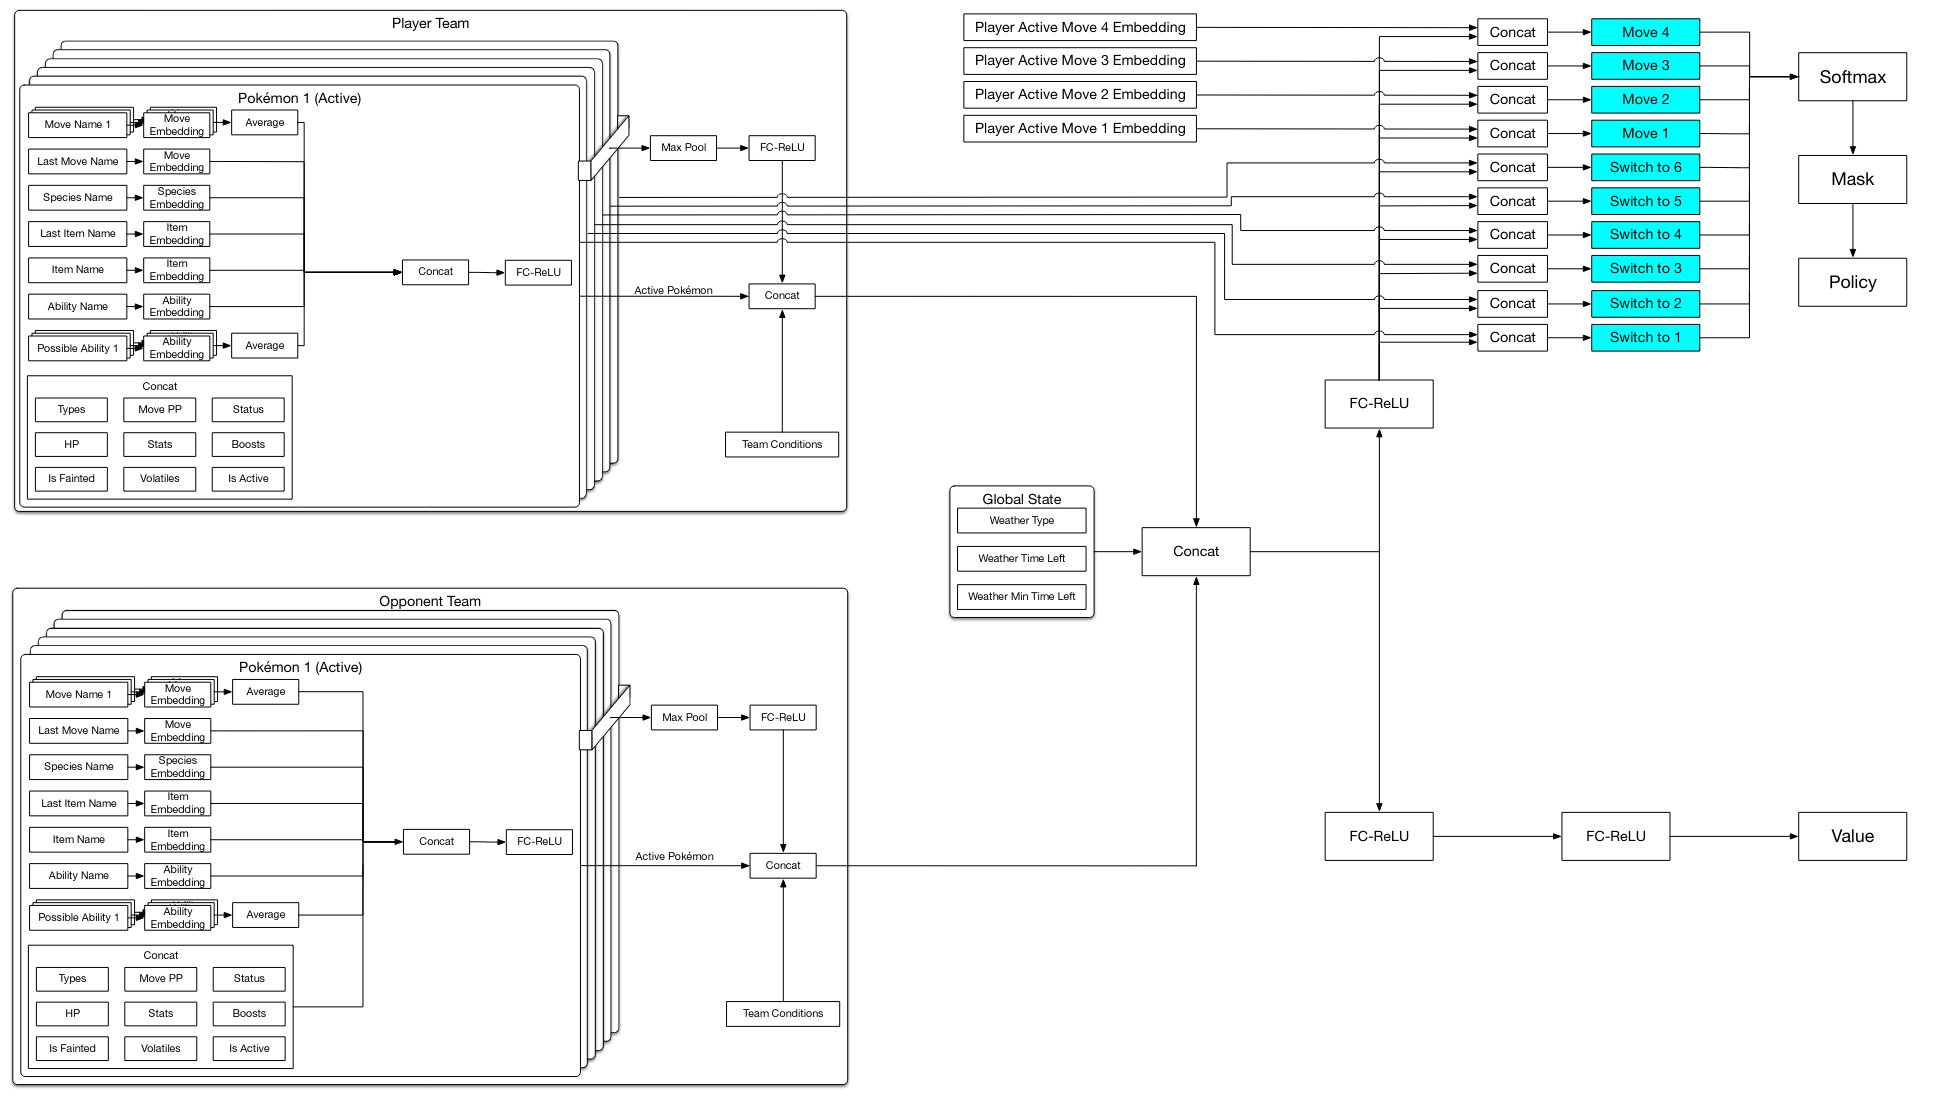
\includegraphics[width=0.9\textwidth]{images/RL-Network-Structure.png}
	\caption{The actor-critic neural network used by the authors in \cite{Lee_Togelius_2017}}
	\label{fig:lee-network}
\end{figure}
The authors point out the following two key design decisions: First, a 128-dimensional entity embedding layer
for each of the categorical variables is used. This enables capturing similarities between different moves,
species and abilities without having to directly model their, often complicated, effects. Second, the
parameters for computing $p$ from above are shared among all $n$ actions. The resulting network is described
by figure \ref{fig:lee-network} and contains 1,327,618 parameters in total \cite{Lee_Togelius_2017}.

\paragraph{Training the network}
Training was done serially: After $m = 7680$ games per iteration, the neural network parameters are updated
using the $2m$ self-play matches as training data to obtain new neural network parameters. A reward
of $+1$ for a win and $-1$ for a loss are assigned at the end of the match. To speed up learning, a 
dense reward signal using reward shaping was constructed. Auxiliary rewards are assigned based on
events that occur over the course of the match. For example, a reward of $-0.0125$ is added when a 
Pokémon of the agent faints, and a reward of $+0.0025$ whenever the player's Pokémon makes a 
super effective move. \\
To update the neural network, the authors use \textit{Proximal Policy Optimization}, which optimizes
an objective function that combines expected reward, accuracy of state value prediction, and a bonus
for high entropy policies. To reduce the variance of policy gradient estimates, \textit{Generalized
Advantage Estimation} is used \todo{Link Paper to both}. \\
After 500 iterations of the training loop, 3,840,000 self-play matches had been played by the neural
network. Training was performed using Google Cloud Platform over the course of 6 days with an 
approximated cost of \$91 USD.

%!TEX root = thesis.tex

\chapter{Approach}
\label{ch:approach}

\section{Basic rules}
\todo{Game is turn based} \\
\todo{Each player has 6 Pokémon} \\
\todo{If a Pokémon has no HP left, it faints} \\
\todo{If all Pokémon of a player fainted, the player loses} 

\section{Battling}
One of the key aspects of the Pokémon game is to battle other Pokémon. In the mainline games, you can 
have up to six Pokémon in your team, also known as party. There is the option to swap a Pokémon with
another Pokémon, but you can't have more than six Pokémon at any point in your team. When playing the 
original Games, you can explore the world to find more Pokémon and use your team to defeat wild Pokémon
and other Pokémon trainer. This thesis however focus on random battles taking place on Pokémon Showdown.
In a random battle, both you and your opponent get a team of six random Pokémon. At the start of the battle,
you know each of your six Pokémon but only the currently active enemy Pokémon. \\
Every turn, both players can choose to either use a Move of their currently active Pokémon or switch
their active Pokémon to another Pokémon. Moves can either deal direct damage to the enemy Pokémon or 
yield other advantages like increasing the damage dealt by the next move. Moves will be covered in more
detail in section \ref{sec:moves}. Each Pokémon has an amount of \ac{HP}. The \ac{HP} of a Pokémon
can be dropped by attacking it with a Move. If the \ac{HP} of a Pokémon drops to zero, it faints and 
can't be used in this battle anymore. A player wins, if all Pokémon of the enemy are fainted. \\
\textit{Note:} In the mainline games there is the possibility to heal or even revive a fainted 
Pokémon during battle using \textit{Healing Items} like \textit{Revive} or \textit{Hyper Potion}.
In competitive Play, only \textit{Held items} like \textit{Leftovers} are allowed. Items will explained
in depth in section \ref{sec:items}.

\subsection{Types}
Pokémon implements a \textit{Rock-Paper-Scissors}-like system. Each Pokémon has eiter one or two of 
18 types. For example, a \textit{Fire}-type Pokémon is weak against \textit{Water}-type Pokémon
whereas a \textit{Water}-type Pokémon is weak against \textit{Grass}-type Pokémon. Lastly,
a \textit{Grass}-type Pokémon is weak against \textit{Fire}-type Pokémon. 
\begin{figure}
	\centering
	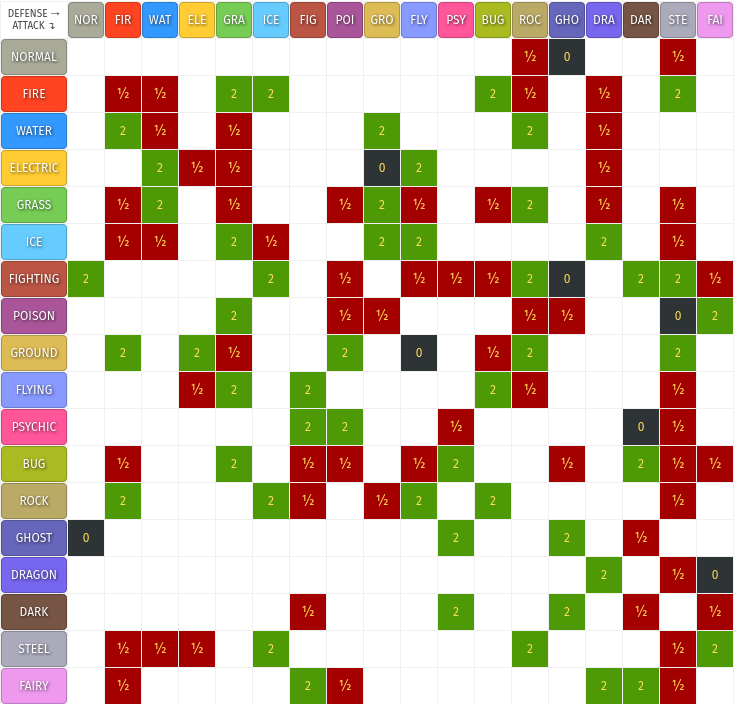
\includegraphics[width=0.7\textwidth]{images/type_chart.png}
	\caption{Pokémon type chart \cite{Pokemondb:Type}}
	\label{fig:type_chart}
\end{figure}
The figure \ref{fig:type_chart} shows how different Pokémon types interact with each other. It is important
to note, that the type modifiers will be multiplied if a Pokémon has two types. For example, a \textit{Fire}-type
attack will deal 4 times the damage against \textit{Parasect} as \textit{Parasect} has the types \textit{Grass} and
\textit{Bug} \cite{Veekun:Parasect}.

\subsection{Moves}
\label{sec:moves}
Moves can either deal direct damage to the enemy Pokémon or yield other advantages, possibly multiple turns 
in the future. \\



\subsubsection{Move Categories}
\todo{Physical and Special moves} 

\subsection{Switching}
\label{sec:switching}

\subsection{Types}
\label{sec:types}

\subsection{Items}
\label{sec:items}

\subsection{Field Conditions}
\todo{Weather conditions} \\

\subsection{Damage calculation}
\label{sec:damage-calculation}
The damage dealt by a move mainly depends on the \textit{level} of the Pokémon
that uses the move, its effective Attack or Special Attack stat, the
opponent's effective Defense or Special Defense stat and the move's effective
power. 

Precisely, the damage is calculated as follows\cite{Bulbapedia:Damage}:
\begin{dmath}
  \text{Damage} = \left(\frac{\left(\frac{2 \times \text{Level}}{5}\right) \times \text{Power} \times \text{A / D}}{50} + 2\right)
	\times Targets
	\times Weather
	\times Badge
	\times Critical
	\times random
	\times STAB
	\times Type
	\times Burn
	\times other
\end{dmath}

The only exception for this are moves that deal direct damage. A list 
of these moves can be found at \cite{Bulbapedia:DirectDamage}.

\subsubsection{Level}
\textit{Level} refers to the level of the attacking Pokémon\cite{Bulbapedia:Damage}. 
In Pokémon Showdown, the level is displayed next to the name of the Pokémon.
\todo{Mainline games leveling}

\subsubsection{A / D}
\textit{A} is the effective Attack stat of the attacking Pokémon if the used move is a physical move,
\todo{Reference to physical moves} \\
or the effective Special Attack stat of the attacking Pokémon if the used move is a special move.
\todo{Reference to special moves}
\\
\textit{D} is likewise the effective Defense stat of the target if the used move is a physical move,
or the effective Special Defense of the target if the used move is a special move\cite{Bulbapedia:Damage}.

There are four moves that use stats from different categories, more Information can be found
at \cite{Bulbapedia:MoveStatDifferentCategories}.

\subsubsection{Power}
Power is the effective power of the used move.
\todo{When is the power not equal to the base power}
The \textit{Base Power} of a move in Showdown can be seen when hovering over a move in the move list. \\
\textit{Note:} The same move will always have the same base power. For example, \textit{Fire Punch} will
always have a base power of 75\cite{Bulbapedia:FirePunch}.

\subsubsection{Weather}
The \textit{Weather} modifier is 1.5 if a \textit{Water-type} move is used during \textit{rain} or a 
\textit{Fire-type} move during \textit{Harsh Sunlight}. The modifier is 0.5 if a \textit{Water-type} move
is used during \textit{Harsh Sunlight} or a \textit{Fire-type} move during \textit{rain} \cite{Bulbapedia:Damage}.
\todo{Reference to weather section}

\subsubsection{Critical}
In the latest Generation, a \ac{CRIT} deals 1.5 times the damage compared to a normal hit.
If the \ac{CRIT} rate is not increased, the chance of landing a \ac{CRIT} is 1/24
\cite{Bulbapedia:CriticalHit}. Increasing \ac{CRIT} rate, as well as other stats, will 
be explained in chapter \ref{sec:boosting}. \\
\textit{Note:} In earlier games, \ac{CRIT}s worked different, see \cite{Bulbapedia:CriticalHit} for
more details.

\subsubsection{Random}
\textit{Random} is a random integer percentage between 85\% and 100\%. Because of this, the same move
may deal different damage in the same scenario \cite{Bulbapedia:Damage}.

\subsubsection{STAB}
\textit{STAB} stands for \textit{Same Type Attack Bonus}. It is a multiplier of 1.5 if the used move
is of the same type as the attacking Pokémon. Otherwise, it is 1.0 \cite{Bulbapedia:Damage}.

\subsubsection{Type}
This is the in section \ref{sec:types} described type modifier \cite{Bulbapedia:Damage}.

\subsubsection{Burn}
\textit{Burn} is 0.5 if the attacking Pokémon is burned, and the used move
is a physical move\footnote{This does not apply if the attacking Pokémon has the Ability \textit{Guts}
or the used move is \textit{Facade}}. Otherwise, it is 1.0 \cite{Bulbapedia:Damage}.

\subsubsection{Other}
The \textit{other} modifier is usually 1. A list of exceptions can be found at \cite{Bulbapedia:Damage}.

\subsection{Effective Stats}
\subsubsection{Boosting}
\label{sec:boosting}
\todo{Boosting critical rate}

\section{Hazards}
An \textit{entry hazard} is a condition that affects a side of the field that causes
any Pokémon that is sent into battle on that side of the field to be afflicted by 
a negative effect. Entry hazards are created by moves, usually status moves
\cite{Bulbapedia:EntryHazards}. \\
\todo{This paragraph is copied word by word from Bulbapedia}
\subsection{List of entry hazards}
Currently, there are five moves that create an entry hazard

\subsubsection{Spikes}
\textit{Spikes} is a \textit{Ground}-type entry hazard that causes the opponent
to lose $1/8$\% of their maximum \ac{HP} when they enter the field. This
effect can be stacked up to three times. Two layers of spikes will deal
$1/6$\% and three layers will deal $1/4$\% of the enemies maximum \ac{HP}. \\
\todo{Removal and Immunity of Spikes}
Spikes are created by the move \textit{Spikes}\cite{Bulbapedia:Spikes}.

\subsubsection{Stealth Rock}
\label{sec:stealthrock}
The move \textit{Stealth Rock} sets an entry hazard around the target Pokémon
causing Pokémon on the target's field to receive damage upon being switched in.
The amount of damage inflicted is affected by the effectiveness of the type
\textit{Rock} against the target. Unlike Spikes, this entry hazard does not stack.
The damage taken from the victim's maximum is denoted in table 
\ref{tab:stealth-rock-damage}\cite{Bulbapedia:StealthRock}.
\begin{table}[h]
	\label{tab:stealth-rock-damage}
	\centering
	\begin{tabular}{|c|c|}
		\hline
		\textbf{Type effectiveness} & \textbf{Damage (Max. \ac{HP}}) \\
		\hline 
		0.25x & 3.125\% \\ 
		\hline 
		0.5x &  6.25\% \\ 
		\hline 
		1x & 12.5\% \\
		\hline
		2x & 25\% \\
		\hline
		4x & 50\% \\
		\hline
	\end{tabular} 
	\caption{Damage dealt to Pokémon by Stealth Rocks\cite{Bulbapedia:StealthRock}}
\end{table}
\textit{Note:} Stealth Rocks can also be created by the move \textit{G-Max Stonesurge}.
This damage-dealing Water-type G-Max move is exclusive to Gigantamax Drednaw
\cite{Bulbapedia:GMaxStonesurge}. \\
\todo{Does this move exist in Showdown}

\subsubsection{Sticky Web}
The entry hazard set by the \textit{Bug}-type move \textit{Sticky Web} lowers the
opponents speed stat by one stage upon switching in \cite{Bulbapedia:StickyWeb}. \\
\todo{Pokémon that are not affected by this}

\subsubsection{Poison spikes}
\label{sec:poison-spikes}
\textit{Poison Spikes} set by the \textit{Poison}-type move \textit{Toxic Spikes}
cause the opponent to become poisoned. If two layers of spikes are set, the
Pokémon instead becomes badly poisoned \cite{Bulbapedia:ToxicSpikes}. \\
\todo{Pokémon not affected} \\
\todo{Explain (badly) poisoning}

\subsubsection{Sharp steel}
This entry hazard works very similar to Stealth Rock described in \ref{sec:stealthrock}.
However, Sharp steel can only be set by the \textit{Steel}-type move
\textit{G-Max Steelsurge} which is the exclusive G-Max Move of Gigantamax Copperhead.
The damage dealt by Sharp steel does not stack, the amount of damage dealt is
based on the Type effectiveness of the \textit{Steel}-type against the target.
Exact damage modifiers can be found in table \ref{tab:sharp-steel-damage}
\cite{Bulbapedia:GMaxSteelsurge}.
\begin{table}[h]
	\label{tab:sharp-steel-damage}
	\centering
	\begin{tabular}{|c|c|}
		\hline
		\textbf{Type effectiveness} & \textbf{Damage (Max. \ac{HP}}) \\
		\hline 
		0.25x & 3.125\% \\ 
		\hline 
		0.5x &  6.25\% \\ 
		\hline 
		1x & 12.5\% \\
		\hline
		2x & 25\% \\
		\hline
		4x & 50\% \\
		\hline
	\end{tabular} 
	\caption{Damage dealt to Pokémon by Sharp Steel\cite{Bulbapedia:GMaxSteelsurge}}
\end{table}
\todo{Unaffected Pokémon}

\subsection{Hazard counterplay}
There are some moves that can remove entry hazards. \textit{Rapid Spin} 
\cite{Bulbapedia:RapidSpin} removes entry hazards from the user's side of the field and
\textit{Defog}\cite{Bulbapedia:Defog} removes entry hazards on both sides of the 
field\footnote{In older games \textit{Defog} would only remove Hazards on the
target's side of the field. But as we only investigate the latest version, this
won't be covered in detail.}. In addition, 
\textit{Court Change}\cite{Bulbapedia:CourtChange} will exchange the entry hazards
on each side of the field, along with other one-sided field conditions.
\todo{What other one-sided field conditions are there?}
If a grounded\footnote{The term \textit{grounded} is used to describe a Pokémon that
can't be affected by damaging \textit{Ground}-type moves and several other associated 
effects\cite{Bulbapedia:Grounded}.}
\textit{Poison}-type Pokémon enters the battle, it will remove Toxic 
Spikes, described in \ref{sec:poison-spikes}, from its side of the field.
Lastly, Pokémon holding the item 
\textit{Heavy-Duty Boots}\cite{Bulbapedia:HeavyDutyBoots} are unaffected by
entry hazards, but grounded \textit{Poison}-type Pokémon can still remove
Toxic Spikes even if they hold the boots\cite{Bulbapedia:EntryHazards}.
There are various exceptions and special cases to hazards. 
\todo{Special cases of hazards}
%!TEX root = thesis.tex

\chapter{Evaluation}
\label{ch:evaluation}
\todo{Lee-Paper: MinMax requires simulation}

\section{Challenges for evaluation}
\label{sec:eval-challenges}

Different researchers use different metrics to evaluate the performance of their agents. 
There are multiple factors that increase the difficulty of properly evaluating the performance.

\subsection{Randomness of battles}
\label{sec:eval-challenges-randomness}
As teams are generated randomly, one player often ends up with a slightly better team than his opponent.
In extreme cases, one player may not even have a chance at winning the battle. While battling
our agent during the evaluation process, one particular game stood out as the first Pokémon of 
\textbf{Player1} was capable of defeating the entire enemy team. \\
The Pokémon of \textbf{Player1} was a \textit{Volcarona} with the following moves:
\begin{itemize}
    \item \textit{Fire Blast}, a damaging \textit{Fire}-Type move
    \item \textit{Quiver Dance}, a \textit{Bug}-Type move that boots the users \ac{SPA}, \ac{SPD} and 
    \ac{SPE} by one stage each.
    \item \textit{Bug Buzz}, a damaging \textit{Bug}-Type move
    \item \textit{Roost}, a move that restores half of the user's maximum \ac{HP}
\end{itemize}
This Pokémon was able to defeat the entire enemy team with little to no possible counter play:
The first enemy Pokémon, \textit{Leafeon}, a \textit{Grass}-Type Pokémon was killed in one hit using
\textit{Fire Blast} after damaging \textit{Volcarona} using \textit{X-Scissor}. \\
Next, \textit{Glalie}, an \textit{Ice}-Type was sent into battle. \textit{Glalie} uses his best move,
\textit{Earth Quake} which brings \textit{Volcarona} to 52\% \ac{HP}. As the enemy does not pressure
\textit{Glalie} much, \textbf{Player1} decided to boost using \textit{Quiver Dance}. Now, \textit{Volcarona}
is faster than his enemy and kills it again in one hit using \textit{Fire Blast}. \\
Then, \textit{Mr. Mime (Galar)} is sent into battle. He fails to pressure \textit{Volcarona} and therefore,
\textbf{Player1} can heal his Pokémon using \textit{Roost} and further boost using \textit{Quiver Dance}. After
defeating \textit{Mr. Mime (Galar)}, \textit{Volcarona} is back to 84\% HP and boosts of 2.5 \ac{SPA},
1.5 \ac{SPD} and 2.5 \ac{SPE}. \\
boosted this high, \textit{Volcarona} can one-shot both the enemy \textit{Volcarona},
\textit{Pheromosa} and the dynamaxed \textit{Scraggy} using \textit{Fire Blast}. \\
To eliminate the impact of these extreme cases, evaluation of agents against other agents 
should be done using multiple hundreds to thousands of games against each other. \\
In order to quantify and better visualize the randomness of battles, we started by generating 
\todo{HOW MANY GAMES IN TOTAL FOR GRAPH} random battles and collected the team information. After
both teams were stored, two \emph{MaxDamage}-agents finished the game to determine a winner.
\todo{Board rating was not done EXACTLY the same way as in the scoring chapter. This uses isCheck!
Scoring does not use isCheck as in the bot itself we only need the score if we have NO check / counter!}
Next,
we determined the matchups for each battle as described in \ref{sec:determine-matchups}. Finally,
the board rating was calculated as follows:
\begin{lstlisting}[language=Python, caption=Calculate Board rating]
  # Amount of counters player 1 has against player 2
  counter_p1_count = sum([sum([
    1 if m.is_counter(m.pokemon_1.species, m.pokemon_2.species)
    else 0 for m in matchups if m.pokemon_1.species == p.species])
    for p in self.team_1])

  # Amount of counters player 2 has against player 1
  counter_p2_count = sum([sum([
    1 if m.is_counter(m.pokemon_2.species, m.pokemon_1.species)
    else 0 for m in matchups if m.pokemon_2.species == p.species])
    for p in self.team_2])

  board_rating = counter_p1_count - counter_p2_count
\end{lstlisting}
Finally, figure \ref{fig:wr-board-rating} displays these results. The figure contains how often what board-rating
occurs (red) as well as the win-rate for the given rating (green).
\begin{figure}[h]
	\centering
	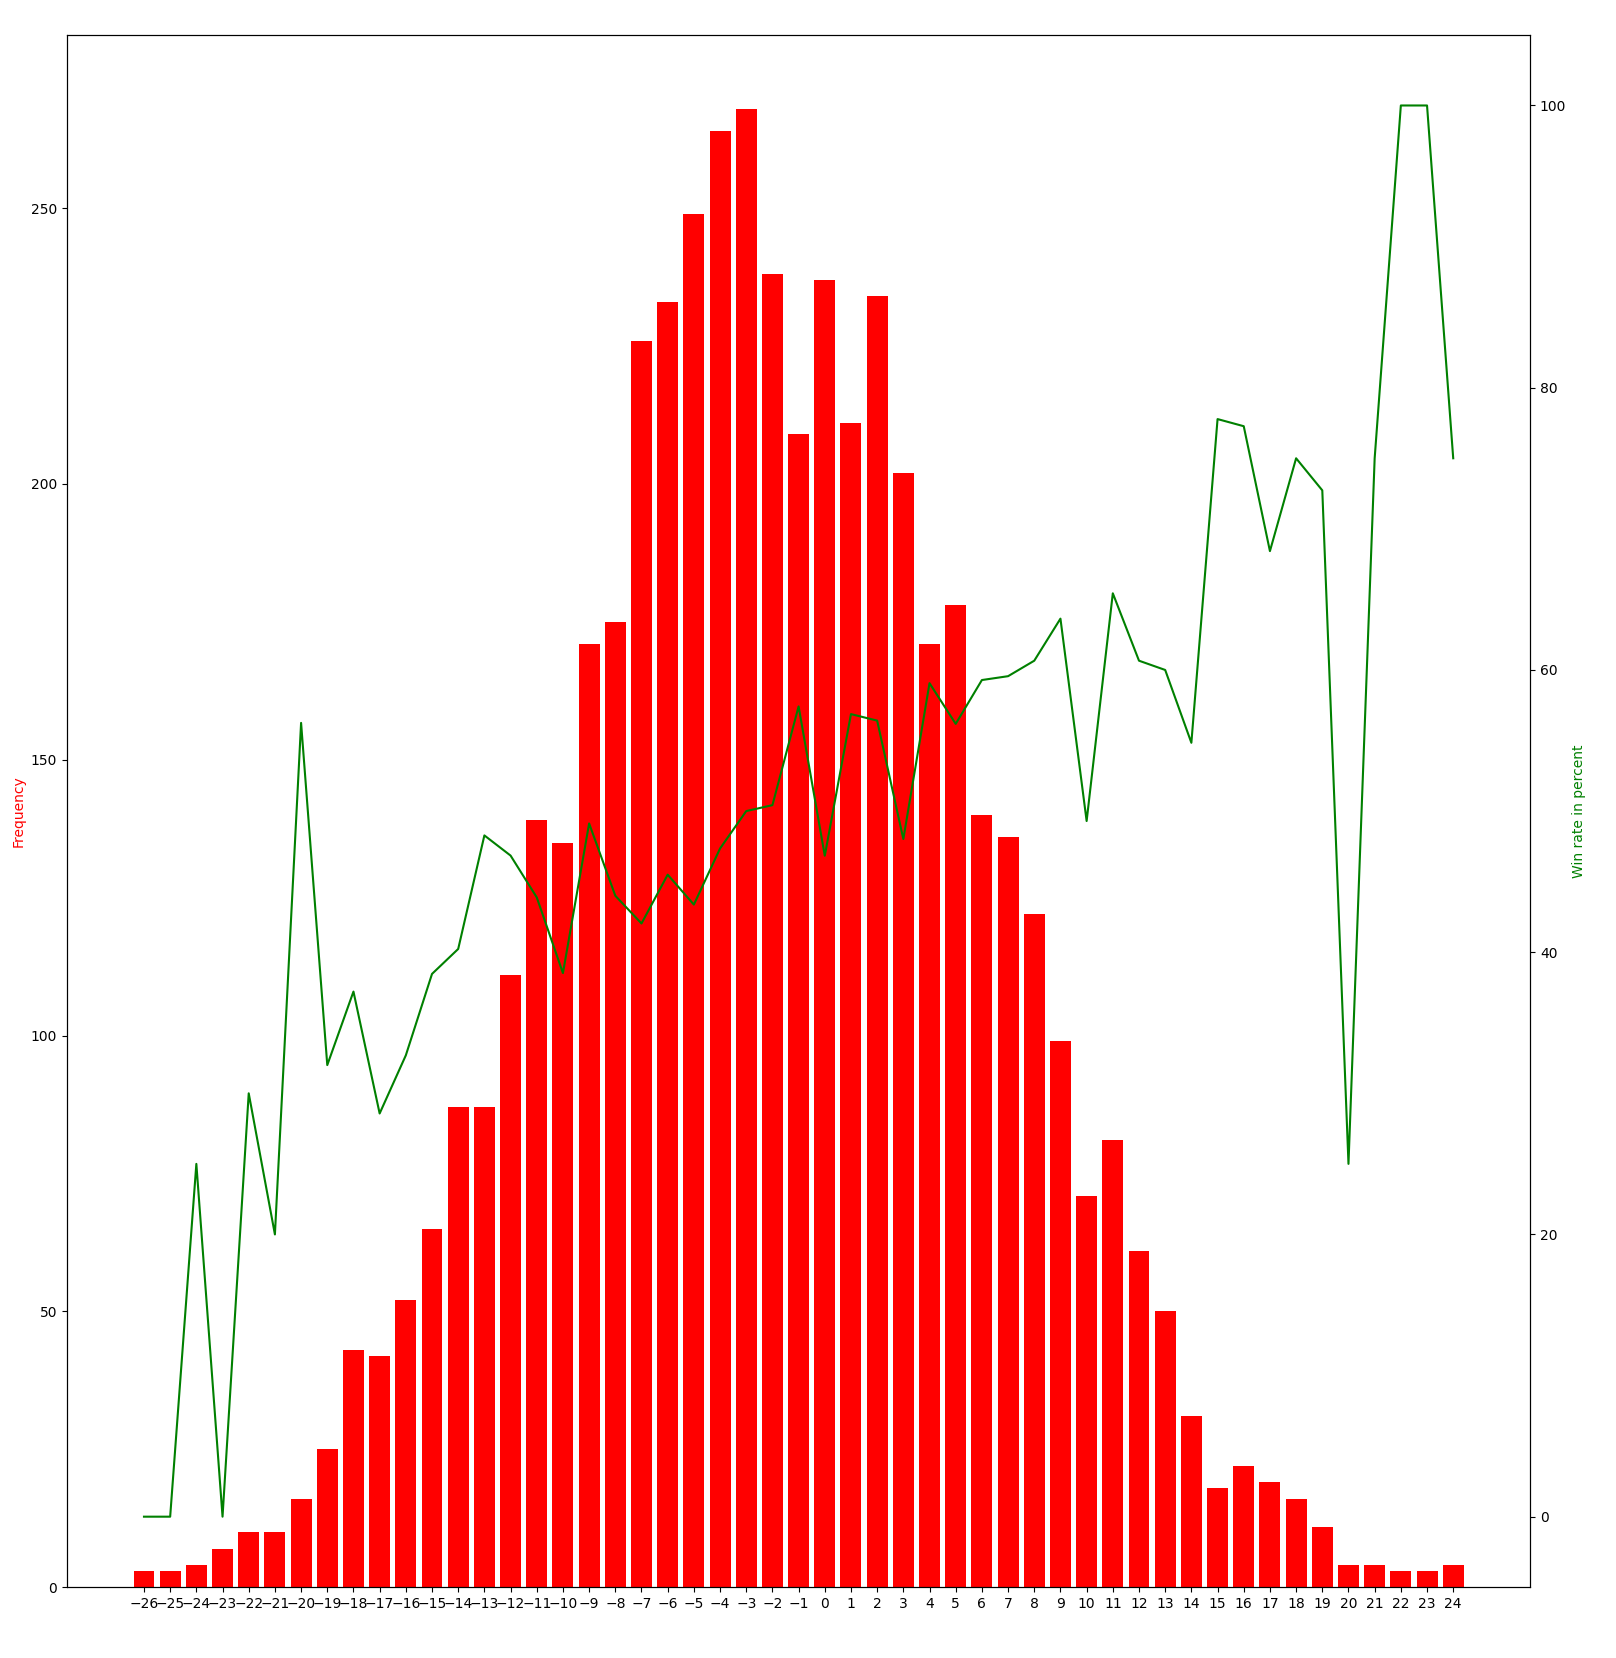
\includegraphics[width=\textwidth]{images/boardrating.png}
	\caption{Win rate for a given board rating}
	\label{fig:wr-board-rating}
\end{figure}
Not only does this figure show a gaussian distribution of how fair games are \todo{Schlechte Formulierung!},
but also that our method of determining matchups works as intended. This is due to the fact that games 
in which we assume the player to be in a bad position also have a win-rate and games with a favorable
board rating show the highest win ratio.

\subsection{Evaluation against human opponents}
As described in \todo{Link Showdown chapter}, Pokémon Showdown allows researchers to use bots on the
ranked ladder. 

\section{Agents}
During this thesis, two different agents were developed, \textit{HerrDonner} and \textit{HerrGewitter}.

\subsection{HerrDonner}
This agent was designed to establish a good baseline and to demonstrate the capabilities of a very
simple rule set. The agent is capable of looking multiple turns into the future. In order to determine
what moves to be used, the Agent generates every possible move combination with the specified amount
of turns into the future and calculates the expected outcome while assuming that the enemy does 
not move at all, similar to the \ac{BFS}-based algorithm described in paragraph \ref{sec:showdown-competition-bfs}. 
No drawback moves that heal the agent, set hazards or field conditions or inflict status conditions
are not considered unless they result in the highest amount of damage dealt. Also, stat changes are 
not taken into account, neither for damage calculation nor for determination of matchups. 
This results in the bot often spamming moves like \textit{Draco Meteor}, a \textit{special} 
\textit{Dragon}-type move that deals a lot of damage but also lowers the
users \ac{SPA} by two stages resulting in the move dealing less damage every time it is used. 
When the agent is forced to switch, it will switch to a check if available. If no check is available,
a counter is sent into battle if one exists. Otherwise, a random Pokémon will be picked. \\
At the start of each turn, \textit{HerrDonner} will check if the current matchup is not favorable, 
a matchup is deemed unfavorable, if the current Pokémon is neither \textit{check} nor 
\textit{counter} to the current enemy. On a bad matchup, the bot will switch to an available 
\textit{check} or \textit{counter}. If neither is available, the bot won't switch and try to
defeat the current opponent with his active team member. \\
Dynamaxing is implemented in a very simple and naive way: The agent will always dynamax the
active Pokémon as soon as more than four enemy Pokémon are known. Lastly, if the
current Pokémon is dynamaxed, the agent will not switch, even if the current matchup is not
favorable. 

\subsection{HerrGewitter}
\label{sec:HerrGewitter}
\textit{HerrGewitter} behaves like described in section \ref{ch:approach}. Here, the most notable
differences between both agents are highlighted, and limitations of this agent are discussed. \\
Firstly, more things are taken into consideration when calculating damage, current stat changes are
taken into consideration as well as status conditions. In addition to that, abilities and items
are considered for damage calculation. Furthermore, recoil from moves, healing both from items
like \textit{Leftovers} ~\autocite{Bulbapedia:Leftovers} and moves like \textit{Recover} aren't neglected
anymore. \\
Switching and the selection of moves is done as described in \ref{ch:approach}. \\
These improvements lead to \textit{HerrGewitter} avoiding mistakes of \textit{HerrDonner}. For example,
this agent will burn a physical attacker using for example \textit{Will-O-Wisp} ~\autocite{Bulbapedia:Will-O-Wisp}
in order to reduce damage taken over the next turns. The agent will also boost and heal itself in favorable
situations which stalls the game and forces the opponent to react. Another major improvement is that the
agent switches out the current Pokémon if stat changes resulted in an unfavorable matchup which is especially
important as stat changes reset on swap. \\
There are still a lot of features that \textit{HerrGewitter} is lacking. 

\paragraph{Weather and Field effects}
The first thing to improve in future versions is to add proper support for weather and field effects in 
the damage calculator as well as in the \textit{MinMax}-Algorithm. Currently, the agent is for example
not aware of the fact that a \textit{Fire}-Type move deals 1.5 more damage during \textit{Harsh Sunlight}.

\paragraph{Hazards}
Currently, the agent will always try to set a non-present Hazard in the early game as this does most 
of the time result in a long term benefit. There are however some notable exceptions to this that 
are not yet implemented:
\begin{itemize}
  \item The agent will always set as many hazards as possible in the early game, even if the current matchup 
  is unfavorable, including always setting up to two layers of spikes. A small test on human players indicated
  that this leads to slightly better results than only setting hazards on good matchups, but due to the very
  small sample size, future work is needed to determine the best strategy for setting hazards.
  \item The agent does not take the damage taken by hazards into account when switching Pokémon. 
  \item The agent will always use \textit{Toxic Spikes} even if the opponent has a \textit{Poison}-Type
  Pokémon on his team that will remove this hazard upon being switched in.
  \item The agent will use Hazards even if the current enemy is known to have a hazard-clearing move like
  \textit{Defog} ~\autocite{Bulbapedia:Defog}
  \item The agent will not clear hazards
\end{itemize}


\paragraph{Choice Items}
As described in section \ref{sec:Important-items} Pokémon holding a \textit{Choice}-item are locked into using always 
the same move until they are switched out. The agent has two major flaws in regard to these items: When the active
Pokémon of the agent is holding a choice item and already locked into a move, the agent is not aware of the fact that
once the Pokémon is switched out, it will regain access to his other moves which leads to an incorrect prediction
for future matchups. As described in \todo{Link chapter about re-determining matchups}, the only matchups re-evaluated
on a given turn are matchups that include one of the currently active Pokémon. The following example illustrates how
this design decision lead to issues on Pokémon with \textit{Choice}-items: \\
In the given scenario, our agent has an active \textit{Garchomp} which is locked into using \textit{Earth Quake}. The 
\textit{Garchomp} also has access to the \textit{Rock}-Type move \textit{Stone Edge}. This turn \textit{Butterfree},
a \textit{Bug / Flying}-Type Pokémon
is sent into Battle. As the \textit{Ground}-Type move \textit{Earth Quake} has no effect on \textit{Butterfree}, the agent will
switch out \textit{Garchomp} for another Pokémon. In the current implementation, matchups for \textit{Garchomp} are not
re-evaluated. While this won't lead to problems in the early game, this results in an incorrect \textit{MinMax} calculation
as for matchups involving \textit{Garchomp} and any non-active opponent, \textit{Garchomp} is still assumed to only have
access to the move \textit{Earth Quake}. In this scenario, the agent would fail to realize that \textit{Garchomp} also
has access to \textit{Stone Edge} and would incorrectly assume Garchomp to loose all matchups against \textit{Flying}-Type
Pokémon. \\
While this behavior rarely effects battle, the agent failing to realize that an enemy is choice-locked has more often a 
negative impact on the battle: If the enemy is known to be choice-locked into \textit{Earth Quake} we can safely switch 
a \textit{Flying}-Type into battle. This applies especcially if the enemy Pokémon is known to have the \textit{Rock}-type 
super effective
move \textit{Stone Edge} as the enemy can't use this move until switched out and back in again. In this scenario, the
agent wrongfully would not prefer to switch in a \textit{Flying}-Type Pokémon due to the thread posed by 
\textit{Stone Edge}. Switching in a Pokémon resisting \textit{Earth Quake} in this scenario forces the enemy to switch
to another Pokémon. This gained turn advantage can either be used to land an extra move on the next opponent, set hazards,
beneficial field conditions, inflict status conditions or boost the current Pokémon.

\paragraph{Damage Calculator}
The current implementation relies on the Pokémon Showdown Damage Calculator. As of now, this open source project does 
only support direct damage dealt by attacking and lacks functionalities like recoil, healing from items and moves. While
we added these features to our implementation, some moves are still not properly implemented. For example, the move
\textit{Counter} has a move priority \todo{Explain move priorities} of $-5$ and works as follows:
If the last mount of damage dealt before the use of \textit{Counter} is greater than zero and was dealt by a 
\textit{Physical}-Type move, \textit{Counter} will do twice as much damage to the opponent. Otherwise, the move
will miss. Additionally, \textit{Counter} has a lot of extra rules regarding other special moves in place 
~\autocite{Bulbapedia:Counter}. Issues like these are especially obvious on \textit{Wobbuffet} as all of his four
most likely moves, \textit{Mirror Coat}, \textit{Encore}, \textit{Counter} and \textit{Encore} are very useful
yet don't deal any damage and are not implemented yet which leads the agent to believe that this Pokémon is bad 
in every possible matchup and has no good use scenarios whatsoever.

\paragraph{Dynamaxing}
\todo{Example in last Pro replay}

\paragraph{Other special cases}
This list contains more currently unhandled cases which will be addressed in future versions:
\begin{itemize}
  \item The Pokémon \textit{Ditto} can transform itself into the Pokémon of the current opponent.
  \item The Pokémon \textit{Zoroark} can transform itself into another team member. 
  \item The ability \textit{Trace} changes the ability of a Pokémon to the ability of his opponent.
\end{itemize}

\paragraph{MinMax}
The \textit{MinMax} algorithm described in paragraph \ref{ref:defeat-phase} only support changes in health
but ignores other important factors such as boosts and status conditions. Therefore, the agent will 
not recognize the possibility to weaken a very strong physical attacker like \textit{Garchomp} by burning
it first and then defeating it with another Pokémon. A simple way to include \ac{BRN} into this algorithm
is to multiply the expected damage dealt by a burned Pokémon with $0.5$. 

\section{Results}
\subsection{Ranked results}
\begin{figure}[h]
  \centering
  \begin{minipage}{.5\textwidth}
    \centering
    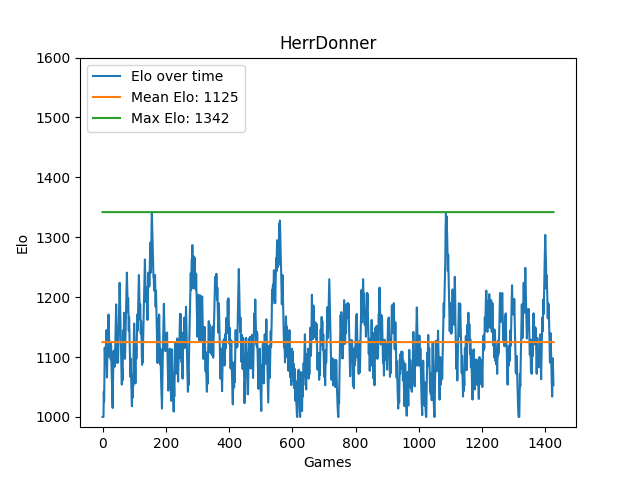
\includegraphics[width=1\linewidth]{images/Donner-Elo-Time.png}
    \captionof{figure}{Elo HerrDonner}
    \label{fig:donner-elo}
  \end{minipage}%
  \begin{minipage}{.5\textwidth}
    \centering
    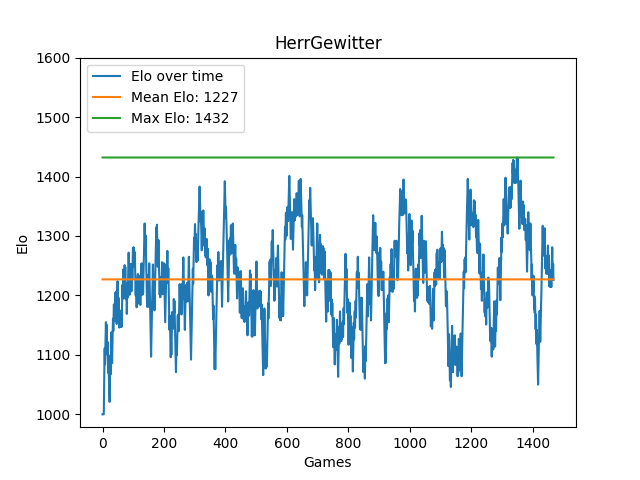
\includegraphics[width=1\linewidth]{images/Gewitter-Elo-Time.png}
    \captionof{figure}{Elo HerrGewitter}
    \label{fig:gewitter-elo}
  \end{minipage}
\end{figure}
\todo{Print this page and check if the figures are to small}
Both agents were evaluated at the same time over the span of multiple days by playing over 1400 ranked games each 
against human opponents on Pokémon Showdown. Figure \nameref{fig:donner-elo} shows the Elo rating of \textit{HerrDonner}
over time, while figure \ref{fig:gewitter-elo} displays the Elo rating of \textit{HerrGewitter}. 
\begin{figure}[h]
	\centering
	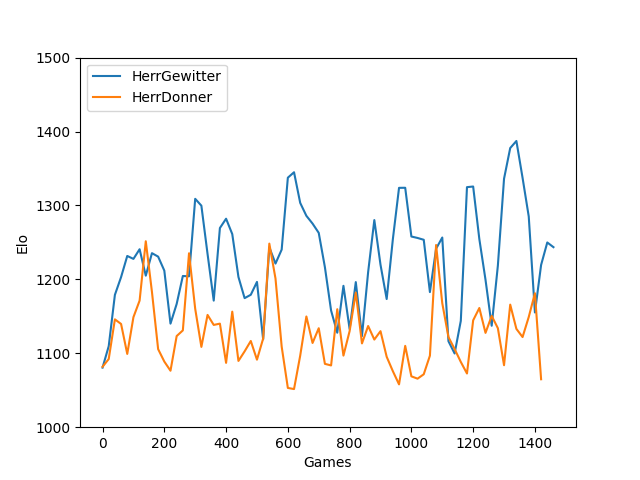
\includegraphics[width=0.7\textwidth]{images/Smoothed-Elo-Time.png}
	\caption{Smoothed Elo}
	\label{fig:elo-smoothed}
\end{figure}
In order to make comparison of both agents more easy, figure \textit{fig:elo-smoothed} shows the smoothed Elo of
both agents over time. Smoothing was achieved by dividing the Elo history in chunks of size 20 and then plotting
the average Elo of each chunk. 
\\\begin{minipage}{\linewidth}
\begin{lstlisting}[language=Python, caption=Smoothing Elo values]
  step = 20
  smoothed_elo = []
  for i in range(0, len(elo_history), step):
      sec = elo_history[i: i + step]
      smoothed_elo += [(i, sum(sec) / len(sec))]
\end{lstlisting}
\end{minipage}
The first thing to note is that \textit{HerrGewitter} has a higher mean Elo ($1227$) as well as a higher max Elo ($1432$)
than \textit{HerrDonner} who achieved an average Elo of $1125$ and peaked at an Elo of $1342$. 
\begin{table}[h]
  \centering
  \begin{tabular}{|l|c|c|c|c|c|c|}
    \hline
     & Random & MaxDmg & Pmariglia & DQN & Donner   & Gewitter  \\
    \hline
    Random                                         & N / A  & -      & -         & 995 / 5   & 992 / 8  & 993 / 7   \\
    \hline
    MaxDmg                                         &        & N / A  & -         & 929 / 71  & 906 / 94 & 951 / 49  \\
    \hline
    Pmariglia                                      &        &        & N / A     & 612 / 388  & -        & 273 / 727 \\
    \hline
    DQN                                            &        &        &           & N / A     & -        & -         \\
    \hline
    Donner                                         &        &        &           &           & N / A    & 580 / 420 \\
    \hline
    Gewitter                                       &        &        &           &           &          & N / A     \\                            
    \hline
    \end{tabular}
    \caption{Battle results of 1,000 games between the agents. \\
    \emph{Pmariglia:}~\autocite{Github:pmariglia-showdown} \\
    \emph{DQN:} As described  in ~\autocite{Huang_Lee_2019}}
    \label{tab:agent-performance}
  \end{table}
\todo{No footnote in table? How to properly format this?}
Table \ref{tab:agent-performance} shows the performance of different agents when directly competing against each other.
It is very important to note that while the agent of~\autocite{Huang_Lee_2019} played against an older version of
against~\autocite*{Github:pmariglia-showdown} than our bot did and is therefore not included in this table as 
this possibly leads to misleading interpretations. 
Each entry displays the results of a thousand games played between both agents. The first number indicates the amount
of games the agent in the current column won. There are a multiple things to point out here: \\
While \textit{HerrDonner} and \textit{HerrGewitter} achieved almost similar results when battling a random agent, 
\textit{HerrDonner} performed notably worse against the \textit{MaxDmg} agent which always picks the move with the
highest base power. Also, \textit{HerrGewitter} only managed to win $58\%$ against \textit{HerrDonner} despite notably
better results against human players \todo{Write about Humans vs. HerrGewitter / Donner}

\section{Investigating Replays}
\begin{itemize}
  \item Bot is really good at switching / using the most damaging move
\end{itemize}
\subsection{Pro Replays}
At the time of writing, \textit{Memezboi69} is the top ranked player on the Pokémon Showdown ladder. I reached
out to him, and he agreed to play three games against \textit{HerrGewitter}. While our agent lost all three 
games, we were able to gain some very interesting insights from these games:

\paragraph{Game One}
In the first game, the bot made a huge miss play that ultimately lead to defeat. The agents \textit{Shuckle} faced a 
\textit{Mr. Mime (Galar)} which had access to \textit{Rapid Spin}, a move that removes hazards. As \textit{Shuckle}
has access to the moves \textit{Sticky Web} as well as \textit{Stealth Rock}, the agent tried to set both hazards
which were immediately removed. In the extra turn, \textit{Mr. Mime (Galar)} boosted its speed stat and slowly
killed his opponent using \textit{Freeze-Dry}. This increased \ac{SPE} lead to an advantage that the bot was
not able to make up for. A future version of the agent will need to include a better hazard routine to prevent
this kind of scenarios.  

\paragraph{Game Two}
Game two was lost due to a lack of answers against the opponents \textit{Gengar}. Prior to sending in this Pokémon,
\textit{Memzboi69} set the entry hazard \textit{Sticky Web} which decreases the \ac{SPE} by one stage on switch in.
After boosting \ac{SPA} by two stages using \textit{Nasty Plot}, \textit{Gengar} was able to defeat the four 
remaining Pokémon of the agent. Further investigation revealed another flaw in the logic of the agent. When switching
in the \textit{Discover Phase} with no check or counter available, the agent ranks all possible options based on how 
much damage they are capable of dealing as described by equation \ref{eq:thread-level} in section \ref{sec:scoring-state}.
If no Pokémon exists that is capable of surviving for more than two turns, the Pokémon with the lowest score will
be sent into battle. In the given scenario, the agent sent out \textit{Klefki} as his last Pokémon. This Pokémon
always has access to either \textit{Thunderwave}, a move that applies \ac{PAR} or \textit{Toxic} that poisons the
opponent. While the chances of winning would still be very low when sending out this Pokémon, bringing in \textit{Klefki}
would have increased the odds. Additionally, the agent did not take the entry hazard into account which lead to
the wrong assumption that \textit{Zamazenta} is faster than \textit{Gengar} and could therefore kill the opponent.
This resulted in \textit{Zamazenta} getting killed in one shot.

\paragraph{Game Three}
The last battle was the closest and ended with \textit{Memezboi69} having only two Pokémon remaining. The agent
even managed to set up a burned \textit{Obstagoon}, boosting \ac{ATK} to stage two and \ac{DEF} to stage three.
Unfortunately, this Pokémon was then killed by \textit{Buzzwole} with the super effective move \textit{Close Combat}.
Even after a lot of investigation, it is hard to determine how this match could have been won by the agent, one 
possibility might have been switching in a \textit{check} to \textit{Buzzwole} and dynamaxing next turn. 
%!TEX root = thesis.tex

\chapter{Conclusion}
\label{ch:conclusion}



%% ----------------
%% |   Listings   |
%% ----------------

\cleardoublepage
\phantomsection
\addcontentsline{toc}{chapter}{\listfigurename}
\listoffigures

\cleardoublepage
\phantomsection
\addcontentsline{toc}{chapter}{\listtablename}
\listoftables

\cleardoublepage
\phantomsection
\addcontentsline{toc}{chapter}{\lstlistlistingname}
\lstlistoflistings

%!TEX root = thesis.tex

\chapter*{Acronyms}
\addcontentsline{toc}{chapter}{Acronyms}

\begin{acronym}
	\acro{HP}[hp]{hit points}
	\acro{ATK}[atk]{attack stat}
	\acro{DEF}[def]{defense stat}
	\acro{SPA}[spa]{special attack stat}
	\acro{SPD}[spd]{special defense stat}
	\acro{SPE}[spe]{speed stat}
	\acro{CRIT}[crit]{critical hit}
	\acro{IV}[iv]{individual values}
	\acro{EV}[ev]{effort values}
	\acro{BRN}[brn]{burn}
	\acro{FRZ}[frz]{freeze}
	\acro{PAR}[par]{paralysis}
	\acro{PSN}[psn]{poison}
	\acro{SLP}[slp]{sleep}
	\acro{RNG}[rng]{random number generation}
	\acro{BFS}[bfs]{breadth-first search}
	\acro{PPO}[ppo]{proximal policy optimization}
	\acro{RPS}[rps]{rock-paprer-scissors}
	\acro{GEN1}[gen1]{generation 1}
	\acro{GEN6}[gen6]{generation 6}
	\acro{GEN7}[gen7]{generation 7}
	\acro{GEN8}[gen8]{generation 8}
	\acro{GEN8RANDBATS}[gen8randbats]{generation 8 random battle}
\end{acronym}


%% --------------------
%% |   Bibliography   |
%% --------------------
\cleardoublepage
\phantomsection
\addcontentsline{toc}{chapter}{\bibname}

\bibliographystyle{ieeetr}
												  
% Use IEEEtran for numeric references
%\bibliographystyle{IEEEtranSA})

\bibliography{thesis}


%% ----------------
%% |   Appendix   |
%% ----------------
\cleardoublepage

%!TEX root = thesis.tex

%% appendix.tex
%%

%% ==============================
%\chapter{Appendix}
%\label{ch:Appendix}
%% ==============================

\appendix

\iflanguage{english}
{\addchap{Appendix}}	% english style
{\addchap{Anhang}}	% german style


\section{First Appendix Section}
		\label{Anhang-Implementierung}
		
\setcounter{figure}{0}
		
\begin{figure} [ht]
  \centering
   ein Bild
  \caption{A figure}
  \label{fig:BPMNBeispiela}
\end{figure}


\dots





%% -------------------
%% |   Declaration   |
%% -------------------
\cleardoublepage
%!TEX root = thesis.tex

\cleardoublepage
\vspace*{20\baselineskip}
\hbox to \textwidth{\hrulefill}
\par
%\iflanguage{english}{english text here}{german text here}

Ich versichere, dass ich die vorstehende Arbeit selbstständig und ohne fremde Hilfe angefertigt und mich keiner anderer als der in den beigefügten Verzeichnissen angegebenen Hilfsmittel bedient habe.
Alle Textstellen, die wörtlich oder sinngemäß aus Veröffentlichungen Dritter entnommen wurden, sind als solche kenntlich gemacht.
Alle Quellen, die dem World Wide Web entnommen oder in einer digitalen Form verwendet wurden, sind der Arbeit beigefügt.

Weitere Personen waren an der geistigen Leistung der vorliegenden Arbeit nicht beteiligt.
Insbesondere habe ich nicht die Hilfe eines Ghostwriters oder einer Ghostwriting-Agentur in Anspruch genommen.
Dritte haben von mir weder unmittelbar noch mittelbar Geld oder geldwerte Leistungen für Arbeiten erhalten, die im Zusammenhang mit dem Inhalt der vorgelegten Arbeit stehen.

Der Durchführung einer elektronischen Plagiatsprüfung stimme ich hiermit zu.
Die eingereichte elektronische Fassung der Arbeit ist vollständig.
Mir ist bewusst, dass nach\-träg\-li\-che Ergänzungen ausgeschlossen sind.

Die Arbeit wurde bisher keiner anderen Prüfungsbehörde vorgelegt und auch nicht veröffentlicht.
Ich bin mir bewusst, dass eine unwahre Erklärung zur Versicherung der selbstständigen Leistungserbringung rechtliche Folgen haben kann.

\vspace*{2\baselineskip}

\textbf{\place, \submissionTime}
\vspace{1.5cm}

\dotfill\hspace*{8.0cm}\\
\hspace*{2cm}(\authorName) %center name with hspace

\thispagestyle{empty}


\end{document}
